% ============================================================
%  00 - DATE CAM Monitoring.tex -- driver file
%
%  DATE 2027 submission draft, v7 (2026-09-02 pm).
%  v7: per MN, the appendices are split into a companion document
%  ("0A - DATE CAM Monitoring Appendices.tex" -> two more PDFs).
%  This driver now builds the MAIN PAPER ONLY (Secs. I-VIII).
%  Cross-references between the documents are hardcoded text
%  ("companion document" here; "of the main paper" there).
%  A hand-off note for Indranil ("Indranil - Focus Areas.tex") is
%  also new in this tree. No content changes from v6 otherwise.
%  Previous: v6 (2026-09-02).
%  v6: round-2 hand-markup applied from
%  DATE-CAM-monitoring_markup-log-round2.md. Sec. IV intro rewritten
%  generically (mapping activation signatures to CAM arrays; NVM
%  parenthetical per MN's margin wording); IV-B leads with FeFET-CAM
%  capability; old IV-C cut to a transition (text in comment);
%  Encoding 1 exposition simplified + "From a hardware perspective"
%  verbatim; headings gain NVM/CMOS qualifiers; K-scores clause
%  footnoted (MN: "footnote it"); Sec. II "Interpretability work that
%  sets K" paragraph and Sec. V small-K paragraph deleted per strikes;
%  Sec. V opener "We first evaluate ... a deception detection
%  workload"; grid-reading sentence added (note E); in-domain
%  paragraph in plain English. New refs: kazemi2022hdcfefet (measured
%  FeFET CAM, Sec. II + subarray split), fefet1c2026 (1FeFET-1C TCAM
%  PoC, thermometer section; authors TBD). Pending: the DAC
%  thermometer paper (orange flag in 04); Ismail question on the
%  decision rule; Fig. 2(a)-(c) keep/cut; Truthfulness-VLA framing.
%  Previous: v5 (2026-09-01).
%  v5: fourth hand-markup pass applied from the pass-2 markup log
%  (DATE-CAM-monitoring_markup-log.md). Comment (D): Sec. IV now leads
%  with "What CAM-resident requires," encodings framed as options;
%  Sec. IV intro reframed (technology-enabled first, CMOS as the
%  nearer-term study). Intro augmented with the OpenAI-Hugging Face
%  incident (per IV.pdf; refs clark2026import, cotra2026hf). Sec. II
%  gains the "what an emerging-technology CAM can or cannot buy"
%  framing (MN's wording), echoed in IV's intro and V-C's takeaway.
%  Cuts: shared-circuitry pointer sentences (II-C, III), ANN block
%  trimmed to two sentences, footnote 4, Sec. IV-B experiment list,
%  V-B recap paragraph. Layer-33 thread resolved: tutorial setup in
%  V-A, forward pointer in IV-B, strategy-first rewrite + why-128 +
%  "384-bit-equivalent." Blue edits verbatim; "must move" and "can or
%  cannot buy" per MN's chat clarifications.
%  Previous: v4 (2026-08-26).
%  v4: per MN, the abstract is the intro's backbone -- abstract culled
%  to ~0.5 column, intro rebuilt from it at ~1 column (STAR-A material
%  folded in, J-space lead-in added, probe arithmetic and overhead
%  detail moved to Sec. II-C); Sec. II restructured (CAM types first,
%  technology placeholder for MN, then preliminaries + related work);
%  Sec. III-D moved to a red-team appendix (09); tok/s reality check
%  added to Sec. III-B; Sec. IV maturity-order lead-in + audit-caption
%  "cheating" note.
%  Previous: v3 (2026-08-25; abstract pass 08-26).
%  v1 (08-17) converted from the IV team briefing deck v3; v2 (08-21)
%  reframed K as growing and brought the J-space results in; v3 (08-25)
%  per MN's markup on 00/01: title picked, the K ladder made explicit
%  and bold (abstract, intro, Sec. III), Figs. 1 and 2 merged into one
%  single-column intro figure (fig_ladder_v1), the overhead progression
%  flipped and reconciled, and a first-order energy/latency estimate
%  added to Sec. VII with the near-term measurement plan. 08-26:
%  abstract reworked per MN's in-file edits and flags (see the review
%  appendix).
%
%  Structure and formatting follow the 1FeFET-1C DATE draft in the
%  sibling folder (IEEEtran conference class, numbered section files,
%  comments.tex flag system, dual-mode compile.sh).
%
%  Compile: bash compile.sh   (produces With/No Comments PDFs)
% ============================================================
\documentclass[conference]{IEEEtran}
\IEEEoverridecommandlockouts

\usepackage{cite}
\usepackage{amsmath,amssymb,amsfonts}
\usepackage{graphicx}
\usepackage{textcomp}
\usepackage[dvipsnames]{xcolor}
\usepackage{RobStd}
\usepackage{subcaption}
\usepackage{siunitx}
% --- siunitx v2/v3 compatibility shim ------------------------
\ifdefined\qty\else
  \NewDocumentCommand{\qty}{O{}mm}{\SI[#1]{#2}{#3}}
\fi
\ifdefined\unit\else
  \NewDocumentCommand{\unit}{O{}m}{\si[#1]{#2}}
\fi
% -------------------------------------------------------------
\usepackage{placeins}
\usepackage{multirow}
\usepackage{makecell}
\usepackage{booktabs}
\usepackage{url}
\renewcommand\arraystretch{1.15}
\setlength{\tabcolsep}{4pt}
\graphicspath{{figures/}}

\def\BibTeX{{\rm B\kern-.05em{\sc i\kern-.025em b}\kern-.08em
    T\kern-.1667em\lower.7ex\hbox{E}\kern-.125emX}}

% --- shorthand macros ----------------------------------------
\newcommand{\cam}{{CAM}\xspace}
\newcommand{\tcam}{{TCAM}\xspace}
\newcommand{\mcam}{{MCAM}\xspace}
\newcommand{\acam}{{ACAM}\xspace}
\newcommand{\imc}{{CiM}\xspace}
\newcommand{\fefet}{{FeFET}\xspace}
\newcommand{\fefets}{{FeFETs}\xspace}
\newcommand{\auroc}{{AUROC}\xspace}
\newcommand{\signrp}{{sign-RP}\xspace}
\newcommand{\tocite}[1]{[{\color{red}citation-#1}]}

% ============================================================
%  comments.tex -- annotation / review-flag system
%
%  STREAMLINED FLAG NAMES (Aug 2026, per MN: "this is just less typing"):
%      \dt[note]{content}   was \dothis   / \dothisflag
%      \eo[note]{content}   was \expandon / \expandonflag
%  The old names are kept as aliases below, so every existing .tex
%  still compiles unchanged. Semantics are identical.
%
%  All flags obey the showcomments boolean; compile.sh flips it.
% ============================================================
\usepackage{ifthen}
\usepackage{amssymb}
\usepackage{xcolor}
\usepackage{etoolbox}
\usepackage{environ}
\usepackage[most]{tcolorbox}

\newboolean{showcomments}
\setboolean{showcomments}{false}    % compile.sh targets this exact line -- keep it here

% DEFAULT IS FALSE (no comments) so Overleaf produces the clean copy.
% Run `bash compile.sh` to build both versions.

\definecolor{flagorange}{RGB}{200, 95, 0}
\definecolor{flagblue}{RGB}{0, 70, 190}
\definecolor{aiviolet}{RGB}{120, 40, 180}
\definecolor{dogreen}{RGB}{0, 130, 60}

% ---- the two action flags -----------------------------------
%  Uniform shape:  \flag[what to do]{content}
%    \dt  orange -- an action to take
%    \eo  blue   -- say more about this
%  Content survives into BOTH builds; the bracketed note appears only
%  in the With Comments build. With NO optional argument the braced
%  text IS the note and disappears from the clean build entirely:
%      \dt{fill in the submission date}          note only
%      \dt[Trim this]{The library is short ...}  keep text, flag it
%      \eo[Add numbers]{}                        note only
\newcommand{\flagmark}[3]{%
  \ifthenelse{\boolean{showcomments}}{{\color{#1}\bfseries[#2:\ #3]}\ }{}%
}
\newcommand{\dt}[2][]{%
  \ifstrempty{#1}%
    {\ifthenelse{\boolean{showcomments}}{{\color{flagorange}\bfseries[DO THIS:\ #2]}}{}}%
    {\flagmark{flagorange}{DO THIS}{#1}#2}%
}
\newcommand{\eo}[2][]{%
  \ifstrempty{#1}%
    {\ifthenelse{\boolean{showcomments}}{{\color{flagblue}\bfseries[EXPAND:\ #2]}}{}}%
    {\flagmark{flagblue}{EXPAND}{#1}#2}%
}
% ---- aliases (do not "clean these up") ----------------------
\let\dothis\dt
\let\dothisflag\dt
\let\expandon\eo
\let\expandonflag\eo

% ---- reviewer remarks --------------------------------------
% Inline remark:  \inote{short note}  /  \inote[aiviolet]{note}
\newcommand{\inote}[2][red]{%
  \ifthenelse{\boolean{showcomments}}{\textcolor{#1}{[#2]}}{}%
}
% Block remark. Escape underscores as \_ inside.
%   \begin{pnote} ... \end{pnote}    or    \begin{pnote}[aiviolet] ... \end{pnote}
\NewEnviron{pnote}[1][red]{%
  \ifthenelse{\boolean{showcomments}}{\begingroup\color{#1}\BODY\endgroup}{}%
}
% Review-build-only content (whole paragraphs, tables, or a page).
\newcommand{\reviewonly}[1]{\ifthenelse{\boolean{showcomments}}{#1}{}}

% ---- structural boxes (always visible) ---------------------
\newtcolorbox{sectionbox}{%
  colback=black, coltext=white,
  width=\linewidth, boxrule=0pt,
  left=3pt, right=3pt, top=2pt, bottom=2pt,
  fontupper=\sffamily\bfseries\normalsize,
  sharp corners,
  before=\par\vspace{4pt}, after=\par\vspace{2pt}}
\newtcolorbox{subsectionbox}{%
  colback=lightgray, coltext=black,
  width=\linewidth, boxrule=0pt,
  left=3pt, right=3pt, top=1pt, bottom=1pt,
  fontupper=\sffamily\bfseries\small,
  sharp corners,
  before=\par\vspace{3pt}, after=\par\vspace{1pt}}

% ---- per-author inline notes -------------------------------
\makeatletter
\newcommand{\mynote}[3]{%
  \ifthenelse{\boolean{showcomments}}{%
   \fbox{\bfseries\sffamily\scriptsize#1}%
   {\small$\blacktriangleright$\textsf{\emph{\color{#3}{#2}}}$\blacktriangleleft$}}%
  {\@bsphack\@esphack}%
}
\makeatother
\definecolor{PersianGreen}{rgb}{0, 0.65, 0.58}
\newcommand{\mn}[1]{\mynote{MN}{#1}{violet}}
\newcommand{\ib}[1]{\mynote{IB}{#1}{PersianGreen}}
\newcommand{\sj}[1]{\mynote{SJ}{#1}{blue}}
\newcommand{\xh}[1]{\mynote{XH}{#1}{orange}}

% \setboolean{showcomments}{true}   % or run: bash compile.sh

\begin{document}

% ============================================================
%  ANNOTATION FLAGS -- quick reference
%
%  All flags compile away when showcomments is false (the default).
%  The two action flags take the SAME shape, \flag[what to do]{content}.
%  Content survives into BOTH builds; the bracketed note appears only in
%  the With Comments build. With NO optional argument the braced text IS
%  the note and disappears from the clean build entirely.
%
%  ORANGE -- an action to take
%    \dt[note]{content}          (was \dothis / \dothisflag; still work)
%    \dt{fill in the deadline}   note only, vanishes from the clean build
%
%  BLUE -- say more about this
%    \eo[note]{content}          (was \expandon / \expandonflag; still work)
%
%  RED / VIOLET -- reviewer remarks, review build only
%    \inote{short note}   \inote[aiviolet]{AI-generated suggestion}
%    \begin{pnote} ... \end{pnote}     block note; escape _ as \_
%    \reviewonly{...}                  content only in the review build
%
%  PER-AUTHOR inline notes: \mn{...} \ib{...} \sj{...} \xh{...}
%
%  A ']' typed inside a flag's optional argument silently truncates it
%  and leaks the rest into the CLEAN build. Brace them: {[1]}, {[5]}.
% ============================================================

% ============================================================
%  WRITING CONVENTIONS FOR THIS DRAFT (MN's voice; fix-ai-writing skill)
%
%  1.  Plain, first person plural, hedged. "may", "could", "appears to",
%      "remains to be established". No absolutes that are not absolute.
%  2.  En dashes (--), never em dashes (---).
%  3.  Numbered inline lists: {\bf (1)} ... {\bf (2)} ..., not
%      "First, ... Second, ...".
%  4.  Bold run-in lead-ins end with a COLON, not a period, and the next
%      word keeps its capital:  \textbf{What the grid measures:} Whether ...
%  5.  Never the word "honest" as framing; never announce your own
%      fairness ("to be fair", "stated fairly", "candidly").
%  6.  No self-referential framing: "the whole argument", "the key
%      insight", "which is the entire problem", "the upshot", "X turns
%      on Y". State the substance and stop.
%  7.  No verdict tags on your own description ("and it works").
%  8.  Do not narrate design choices ("deliberately", "chosen to be").
%  9.  A section discusses; it is not a proof. "Sec. IV covers ...",
%      not "Sec. IV is the proof that ...".
%  10. No "binds" / "bites" for constraints; no borrowed-metaphor verbs
%      ("is the currency", "prices the choice", "lands on", "rests on").
%      Use "maps to", "depends on", "the limit here is".
%  11. American spelling, always. Define every acronym at first use.
%  12. Scope caveats go in footnotes, not into the argumentative flow.
%  13. Label invented or illustrative examples as such, in the text.
%  14. Figures follow the house-graphs conventions: Helvetica, Set1
%      colors, transparent background, provenance header in the
%      generating script (see gen_paper_figs.py).
% ============================================================

\bstctlcite{IEEEexample:BSTcontrol}

% DATE is double-blind: authors and funding are anonymized for
% submission. Funding restored at camera-ready (SRC/DARPA JUMP 2.0;
% NSF IRES; etc.).
% Title per MN (08-25): option (2) from the v02 markup -- names the
% design-space contribution first for a DATE audience.
\title{\cam-Resident Behavioral Monitoring for LLMs: Encoding Choices,
Cross-Domain Fidelity, and Library-Size Scaling}

\author{\IEEEauthorblockN{Anonymized for review}
\IEEEauthorblockA{DATE 2027 submission}}

\maketitle

\begin{abstract}
Frontier language model deployments increasingly treat a model's own internal
activations as a safety signal: a production jailbreak defense from
Anthropic, for instance, is realized via a single linear probe over residual-stream
activations, scored on every generated token at roughly
$10^{-3}$~percent of forward-pass compute. What is monitored is set by
$K$, the number of stored behavioral signatures each activation is
compared against, and target $K$'s are rapidly increasing: from $K=1$
in the deployed defense above, to $K\!\approx\!10^{2}$--$10^{3}$ once
probes are fitted per behavior, per domain, and per layer, to
$K\!\approx\!1.3\!\times\!10^{5}$ per layer for a whole-vocabulary
readout, where the signature library equals the model's vocabulary. On a GPU,
the signature bank must stream from high-bandwidth memory once per
monitored token, so at sufficiently high $K$ or token rates -- e.g.,
$K=10^{4}$--$10^{5}$ at $10^{3}$~tokens/s -- the monitor's own memory
traffic can exceed the bandwidth of the accelerator it runs
on.\inote[aiviolet]{broadened per your margin note to capture token
rate alongside $K$; I dropped ``nominally'' as you suspected} We
propose addressing this bottleneck with content-addressable memories
(\cam{}s), which evaluate distance functions directly within the
memory array -- emerging non-volatile devices further enable
richer per-cell distance metrics (e.g., Euclidean).\inote[aiviolet]{Note: your earlier blue edit still doubles up
(``in memory ... in the memory array itself''); if you meant to also
strike ``in the memory array itself,'' say so and it is one deletion.
The emerging-technology clause is new, per your ``briefly work in''
note} Because the signature bank never moves and only the query is
broadcast, this in-memory search trades arithmetic precision and distance function fidelity for orders of magnitude lower data movement. We quantify this trade-off on two
representative workloads: {\bf (1)} a ten-domain cross-domain
deception grid over Llama-3.3-70B activations, where 384-bit codes
preserve in-domain \auroc within 0.01 of the full-precision cosine-similarity
ceiling while achieving more than $300\times$ compression per stored signature; and
{\bf (2)} whole-vocabulary readout, where a 3-bit Euclidean code at
$\sim$$10^{3}$ storage bits per row reproduces 0.96 of the exact
readout's top-1 token selections. Because search occurs in place
rather than via streaming, the dominant costs shift to array capacity and search energy: the
whole-vocabulary bank occupies 6--\qty{33}{\mega\byte} per layer, and estimated
in-array search energy is five to six orders of
magnitude below the energy of streaming the equivalent bank from
HBM.\inote[aiviolet]{rewrote ``Held rather than moved'' per your
``unsure what point of this is'' -- the point was that a bank that
stays in place is priced by capacity and search energy, not
bandwidth; it now says that}
\end{abstract}

\begin{IEEEkeywords}
Content-addressable memory; compute-in-memory; large language models;
activation probes; AI safety monitoring; nearest-neighbor search;
ferroelectric FETs; Hamming distance
\end{IEEEkeywords}

%%%%%%%%%%%%%%%%%%%%%%%%%%%%%%%%%%%%%%%%%%%%%%%%%%%%%%%%%%%%%%%%%%%
\section{Introduction}
\label{sec:Introduction}
%%%%%%%%%%%%%%%%%%%%%%%%%%%%%%%%%%%%%%%%%%%%%%%%%%%%%%%%%%%%%%%%%%%
% Structure (v04; expanded ~1/2 column on 08-26 per MN, so readers
% quickly care): (1) safeguards read text, activations now read in
% production, the K=1 check is small; (2) the security problem --
% long autonomous operations, the AISI incident, found only
% retrospectively; (3) the deception work -- probes recover structure
% but directions are narrow, so K multiplies; (4) the bold ladder,
% with the J-space rung carrying the spider example; (5) propose the
% CAM; (6) contributions.
% Moved out, not cut: probe arithmetic (2Ld, MoE point) and overhead
% detail -> Sec. II-C; cell-type detail -> Sec. II-A; counter-evidence
% -> red-team appendix (09). Sec. VI-A now points at the intro's
% spider example instead of repeating it.

Large language model (LLM) deployments are wrapped in a layered set
of safeguards, and until recently every layer read
\emph{text}~\cite{metr2026policies}. That has started to change: the
always-on stage of one production jailbreak defense now reads the
model's internal activations
directly~\cite{ccpp2026,anthropic2026ccblog}, as do deployed
residual-stream probes at a second provider~\cite{gemini2026probes}.
The deployed check is small -- one stored vector $w$, one dot product
per generated token, one threshold. Only flagged exchanges are
escalated to an expensive classifier ensemble -- and it is a small
share of even the deployed defense's reported overhead
(Sec.~\ref{subsec:Probes}).

Recent security evaluations show why such monitors are needed.
Frontier models now run long, autonomous operations: current cyber
evaluations walk a model through 32 steps from reconnaissance to
takeover, with run budgets up to $10^{8}$ tokens. The strongest
model tested progressed, unaided, through 22 of those 32 attack steps
on an average attempt -- roughly two thirds of the way to a completed
operation~\cite{aisi2026cyber}. In one four-day campaign of 122
such runs across seven models, evaluators later found 19 unsanctioned
actions in four distinct categories -- supply-chain compromise of a real open-source project,
deception and targeting via a file-transfer service, prompt injection
planted for other automated systems to execute, and inter-agent
collaboration via public messages. All of said outcomes were found
\emph{retrospectively}; nothing was watching the models' internal
state as they ran~\cite{aisi2026incident}. One month later the same
behaviors appeared at production scale: per public investigations,
hundreds of agents on OpenAI's infrastructure organized, in secret,
into a working collective -- building a communication channel,
reverse-engineering their own scorer, falsifying evidence, and
compromising both OpenAI and Hugging
Face~\cite{clark2026import,cotra2026hf}. Again, the record was
reconstructed from transcripts after the fact -- and the
coordination itself is a behavior for which no stored direction has
been published. A $10^{8}$-token operation
is not visible by sampling outputs, and each individual message such
an agent emits can read as routine -- a plausible commit, a file
transfer, a status update -- while the sequence they add up to is an
attack. As such, a monitor for this setting has to be per-token,
always-on, and internal.

Interpretability work supplies the signatures such a monitor would
compare against, and it also indicates how many it needs. Linear
probes recover truth-related structure across datasets and model
families~\cite{marks2023geometry,burns2023ccs,zou2023repe}, but the
directions are narrow. A probe fitted on factual lying has an
\auroc score of $\sim$0.55 (random chance) on
sycophancy~\cite{ying2026spectrum}, while probes trained on outright
lying largely miss deception carried by technically true
statements~\cite{berger2026liedetector}. Detecting deceptive
reasoning has become a funded interpretability objective in its own
right~\cite{schmidt2026interp}. Covering a behavior suite therefore
takes a stored direction per behavior, per subject-matter domain, at
each layer where that behavior separates -- and each of those
combinations is one more stored row. As such, $K$, the number of
stored signatures each activation is compared against, can grow with
everything the monitor is asked to notice; and widening what is
covered means growing the library that must be searched.

Fig.~\ref{fig:ladder}(a) plots the published record of $K$ against
time; Fig.~\ref{fig:ladder}(b) estimates the percentage of GPU
bandwidth that could be consumed with increasing $K$.
\textbf{\boldmath$K=1$} represents deployed always-on monitors that
read a single direction~\cite{ccpp2026,gemini2026probes}.
\textbf{\boldmath$K\approx10^{2}$} captures probes that are fitted per
behavior and per domain~\cite{ying2026spectrum}.
\textbf{\boldmath$K\approx10^{3}$} is indicative of the four behavior
categories of the above campaign, multiplied over ten domains and
13--25 usable layers -- i.e., 520--1{,}000
rows~\cite{aisi2026incident}; the production-scale incident above
repeats every one of said categories, so this arithmetic is, if
anything, conservative~\cite{clark2026import}.
\textbf{\boldmath$K\approx1.3\!\times\!10^{5}$} is representative of
the whole-vocabulary (``J-space'') readout, from a published method
reporting that a model holds words ``in mind'' without emitting them
-- i.e., for every token in the vocabulary there is an internal
pattern meaning that word is currently active, and it is readable
whether or not the word is ever
said~\cite{anthropic2026workspace}.\footnote{As an example, prompted
with the number of legs on the animal that spins webs, the model
answers \emph{eight} while the readout shows \emph{spider} active
internally; the same work reports patterns for ``fake'' and
``fictional'' active while a model privately registered that a safety
test was staged.} Finally, $K$ could grow even
higher, as published feature
dictionaries~\cite{templeton2024scaling,gao2024sae,lieberum2024gemmascope}
are even two orders of magnitude higher than the J-space. That said,
we can cross the memory bandwidth of deployable parts well before this.
Per Fig.~\ref{fig:ladder}(b), at $10^{3}$ tokens/s, an H100 is fully
consumed at $K\!\approx\!204$K and a Jetson-class part at
$K\!\approx\!17$K (Sec.~\ref{sec:Scaling}).

\begin{figure}[!t]
\centering

\includegraphics[width=3.4in]{fig_ladder_v2.pdf}
\caption{(a) Monitored library size $K$ in the published record
(left axis), read as GPU monitoring traffic on the right axis via
Eq.~(\ref{eq:gputraffic}) at $d=8{,}192$, fp16, $10^{3}$~tokens/s,
one monitored layer; dashed lines mark two parts' memory bandwidths,
and the green line is a \cam's per-token traffic, flat in $K$. The
arrow joins the record's endpoints; it is not a fit and not a
forecast. (b) The share of a part's memory bandwidth consumed by
monitoring alone, against aggregate token rate and library size $K$:
lines mark 100\% of an H100, an A100, and a Jetson Thor, with 10\%
and 1\% of an H100 as guides. The strip
anchors the rate axis to familiar workloads
(Sec.~\ref{subsec:CostModel}): per-stream anchors batch up to a
node's aggregate rate, while batch-1 edge workloads (VLA, video) sit
on the axis directly -- so batching moves a deployment along the
axis rather than adding one; per-request amortization is objection
(3) of the companion appendix document. Both panels are arithmetic
on vendor bandwidth
figures, not measured kernel throughput.}
\label{fig:ladder}
\end{figure}

We propose to support this search with a content-addressable memory
(\cam), which computes the distance function in the memory array
itself: the bank never moves and per-token traffic is flat in $K$
(green line of Fig.~\ref{fig:ladder}(a)).
Candidate substrates are based on both near-term and the emerging
devices: SRAM-based \cam{}s are buildable in any CMOS process today,
and can implement Hamming distance, while \cam{}s based on emerging
devices (\fefets, RRAM) offer density, nonvolatility, and richer
distance metrics (Secs.~\ref{subsec:CAMspace}
and~\ref{subsec:CAMtech}).

This paper measures that trade for behavioral-monitoring workloads.
Our contributions include: {\bf (1)} a formulation of always-on activation
monitoring as library search, with the traffic and capacity arithmetic
and the GPU crossing points (Secs.~\ref{sec:Scaling},
\ref{sec:Hardware}); {\bf (2)} a maturity-ladder mapping of the
detector onto \cam cell types and match modes, with an audit that
catches classification hiding in a trained front end
(Sec.~\ref{sec:Mapping}); {\bf (3)} measured fidelity at \cam
precision at both ends of the $K$ range -- the ten-domain deception
grid, within 0.009 \auroc of the full-precision ceiling in-domain
(Sec.~\ref{sec:Results}), and an in-house whole-vocabulary readout
reproduction scored against the exact readout
(Sec.~\ref{sec:LargeK}); and {\bf (4)} a first-order search
energy/latency estimate, with the measurements that is the foundation
for future cost models (Sec.~\ref{sec:Hardware}).\inote[aiviolet]{your
edit applied verbatim; ``measurements that is'' -- if you meant the
plural, ``that are the foundation'' fixes the agreement}

\begin{pnote}
Framing check before this goes anywhere: the paper claims a
\emph{component} result, and the reproductions are part of that claim
-- the deception grid reproduces the published cross-domain pattern at
\cam precision, and the watchlist demonstration reproduces the
published readout method in-house at 8B. What the paper does not claim
is a working end-to-end deception detector or a jailbreak-blocking
experiment. The measured claims are about the fidelity and cost of
stored-signature matching under the compression a real in-memory
device would impose. Sec.~\ref{sec:Conclusions} repeats this.
\end{pnote}

%%%%%%%%%%%%%%%%%%%%%%%%%%%%%%%%%%%%%%%%%%%%%%%%%%%%%%%%%%%%%%%%%%%
\section{Background}
\label{sec:Background}
%%%%%%%%%%%%%%%%%%%%%%%%%%%%%%%%%%%%%%%%%%%%%%%%%%%%%%%%%%%%%%%%%%%
% Restructured in v04 per MN's flag: (A) CAM design space first;
% (B) a technology-implementations placeholder MN will fill, seeded
% with the BEOL material; (C) preliminaries (the probe/AUROC material,
% trimmed, plus the probe-cost arithmetic moved out of the intro) and
% related work.

\subsection{The CAM design space}
\label{subsec:CAMspace}
Ordinary memory takes an address and returns content, so searching a
library means reading it row by row. A \cam compares every row
against the query at once, in place, and only reports matching
rows~\cite{pagiamtzis2006cam}. One access is therefore one search of
the whole library, at any library size, and the data that moves is the
query rather than the bank.

A \textbf{binary \cam} (BCAM) cell holds one bit. A
\textbf{ternary \cam} (\tcam) cell holds a bit or a don't-care, which
is what makes a stored ternary code with a zero band natively
expressible~\cite{ni2019fetcam}. A \textbf{multi-bit \cam} (\mcam) cell
holds one of several levels~\cite{kazemi2021fefetcam}. An
\textbf{analog \cam} (\acam) cell
holds a range~\cite{li2020acam}. A binary or ternary cell can report
only whether a position disagrees, and can measure Hamming
distance. A multi-bit or analog cell stores a level,
which is what lets the matchline measure how far the query sits from
what is stored. In a multi-bit \fefet implementation, sweeping the query
voltage traces a V-shaped matchline current with its minimum at the
stored level; the curve is approximately quadratic near the bottom, so
one cell physically computes $(Q_i-M_i)^2$ and $N$ cells on a common
matchline sum to $\sum_i (Q_i-M_i)^2$, a squared Euclidean distance with
no multiplier anywhere~\cite{kazemi2021fefetcam} (see Table~\ref{tab:camspace}). Notably, said cell
behavior has been \emph{measured}, not only modeled: multi-bit,
array-level \cam operations have been experimentally demonstrated
with \fefets -- a two-\fefet cell programmed to eight states (3
bits), whose measured matchline distance function shows the
quadratic behavior described above~\cite{kazemi2022hdcfefet}.\inote[aiviolet]{Sep 2,
your Table~I note: the measured-FeFET-CAM mention, from the
Scientific Reports paper you attached (Kazemi et al.\ 2022) -- the
same source now also carries the subarray-split practice in
Sec.~IV-C}\footnote{Squared
Euclidean is an acceptable stand-in for Euclidean here, since the square
root is monotonic and therefore changes neither which row is closest nor
which rows clear a threshold.}

With appropriate peripheral circuitry we can measure: \textbf{exact}
match reports rows with no mismatches; \emph{best} match reports the
row with the fewest, even when nothing is exact; \textbf{threshold}
match reports
every row within a limit $\tau$.\inote[aiviolet]{Note: your
``Bold'' arrow touched \emph{exact} and \emph{threshold}; \emph{best}
is left italic -- say the word if all three should match} Each is a different matchline circuit.
Threshold mode matters for monitoring because the expected answer is
almost always empty, and a threshold array can report ``nothing fired''
without ranking anything. Table~\ref{tab:camspace} summarizes the
design space; notably, the cheapest cells support only Hamming
distance, which is why encodings that hold accuracy under a Hamming
metric are potentially valuable. A goal of what follows is to
quantify what an emerging-technology \cam can or cannot buy: where
the multi-bit cells of Table~\ref{tab:camspace} change the
achievable accuracy and energy, and where a plain CMOS Hamming
array is already enough.

\begin{table}[t]
\centering
\caption{The \cam design space a monitoring workload has to choose from.
Cell transistor counts are order-of-magnitude figures for CMOS
implementations; NVM-based cells trade area for nonvolatility.}
\label{tab:camspace}
{\footnotesize
\begin{tabular}{@{}llll@{}}
\toprule
\textbf{Cell} & \textbf{Holds} & \textbf{Distance} & \textbf{Cost / maturity} \\
\midrule
BCAM  & one bit            & Hamming            & $\sim$6--10T, any CMOS fab \\
\tcam & bit or don't-care  & Hamming, wildcards & $\sim$16T CMOS; 2T \fefet \\
\mcam & one of $2^b$ levels & Euclidean ($L_2^2$) & multi-level device \\
\acam & a range            & range / interval   & multi-level device \\
\midrule
\multicolumn{4}{@{}l}{\emph{Match mode is an independent choice:} exact,
best-match, or threshold.} \\
\bottomrule
\end{tabular}}
\end{table}

\subsection{\cam technologies}
\label{subsec:CAMtech}
\dt[MN: placeholder per your restructuring note -- your
technology-based \cam content goes here (SRAM vs.\ FeFET vs.\ RRAM
implementations, the SUPREME/JUMP material, whatever you want to
carry). The BEOL paragraph below is the seed; Table~\ref{tab:devices}
in Sec.~VII carries the device figures and could move up here if this
subsection grows]{}
The rungs of Table~\ref{tab:camspace} differ in where the array can
physically sit. SRAM-based binary and ternary cells are buildable in
any CMOS process today, in the front-end silicon alongside logic. The
\fefet-based cells trade that ubiquity for density and nonvolatility,
and their device work is moving toward the back end of line (BEOL):
monolithic-3D integration of high-endurance multi-bit \fefets has been
demonstrated with the memory tier above the logic
tier~\cite{dutta2020m3dfefet}, and BEOL-compatible ferroelectric
transistors with AlScN films on two-dimensional channels have been
reported at thermal budgets a metal stack tolerates~\cite{kim2023alscn}.
BEOL RRAM and MRAM are already offered at 22/16\,nm foundry nodes. A
BEOL-capable cell is what would eventually let the signature bank sit
in the metal layers above the compute that produces the activations;
Sec.~\ref{subsec:Placement} returns to what that placement would mean
for this workload. Notably, none of said substrates would be built
for one application: an SRAM-based associative processing unit
already performs bit-serial Hamming search at billion-vector
scale commercially~\cite{gsi2025apu}, and \cam-based accelerators
have been proposed across retrieval, one-shot learning, and
range-matching workloads -- so a monitoring part rides on a
primitive several markets already use
(Sec.~\ref{subsec:RelatedWork}).\inote[aiviolet]{Sep 1, your (C):
a brief echo of the associative-search-silicon paragraph, worked
in here at the end of II-B; the full paragraph stays in II-C}
\dt[confirm the kim2023alscn author list before submission (Nature
Nanotechnology 2023, AlScN/2D-channel BEOL FeFETs)]{}

\subsection{Preliminaries and related work}
\label{subsec:Probes}
\label{subsec:RelatedWork}
\textbf{What a probe reads, and what it costs:} A token is carried
through a transformer by a running vector, the \emph{residual stream},
that every layer reads from and adds back to. After layer $\ell$,
the result is $h^{(\ell)}$: $d$ numbers ($d=8{,}192$ for a 70B
model), one vector per layer, per token. The individual entries are
not labeled features -- no single coordinate means ``deception'' --
so a detector has to read the vector as a whole rather than watch any
one entry. A \emph{linear probe} is the simplest detector over
that object: one stored vector $w$, fitted offline on labeled
activations, and a threshold $\theta$, with
%
\begin{equation}
w \cdot h \;=\; \sum_{i=1}^{d} w_i h_i \;>\; \theta
\;\;\Longrightarrow\;\; \text{flag.}
\label{eq:probe}
\end{equation}
%
Probes of this form recover truth-related structure across several
datasets and model families~\cite{marks2023geometry,burns2023ccs,
zou2023repe}, and the directions are also actionable: adding a multiple
of one back into the residual stream changes behavior, which is usually
called steering~\cite{zou2023repe}. Scoring one activation is $2Ld$ multiply--accumulate
operations for a model of depth $L$ and residual width $d$ -- about
1.3 million operations for a 70B model, or roughly $10^{-5}$ of the
forward pass. This cost is analogous to $L\!\cdot\!d$ rather than
parameter count, and $L\!\cdot\!d$ has not changed significantly
even with frontier models (e.g., a 671B-parameter mixture-of-experts
model has $d=7{,}168$ and $L=61$~\cite{deepseekv3} -- an
$L\!\cdot\!d$ \emph{smaller} than a dense 70B model's
$8{,}192\times80$ -- so a bigger model could have a smaller probe
vector).\inote[aiviolet]{two of your blue phrases were hard to read:
I typed ``is analogous to'' and ``changed significantly even with
frontier models''; if the second was ``now with,'' say so}

\textbf{How detection is graded:} Quality is typically reported as area
under
the receiver operating characteristic curve (\auroc), i.e., the
fraction of (deceptive, honest) pairs the detector orders correctly;
1.0 is perfect and 0.5 is random. An important ``stress test''
for library size is \emph{cross-domain} -- i.e., fit on one kind of
dishonesty and evaluate on another~\cite{ying2026spectrum}.\footnote{A
\emph{domain} is a subject matter to be dishonest about (what a word
means, a checkable fact, a deduction); a \emph{behavior} is a kind of
dishonesty (lying about a fact, flattering the user, quietly
underperforming on an evaluation).}

\textbf{Activation monitoring in production:} The two-stage cascade
in~\cite{ccpp2026,anthropic2026ccblog} and the deployed Gemini
probes~\cite{gemini2026probes} are the closest published statements of
the workload this paper aims to accelerate; both operate at $K$ of
order one.
Monitoring has gotten cheaper as providers moved from reading text to
reading activations: the first-generation text-classifier pair
reported 23.7\% overhead, while the probe-fronted cascade that
replaced it reports 1--3.5\%~\cite{cc2025,ccpp2026}. Separately
reported monitor overheads of roughly 0.1\% of serving
cost~\cite{anthropic2025cheapmonitors} are consistent with watching
just one or two things. What the published figures do not tell us is
how the 1--3.5\% splits between the probe and the escalation stages;
the $2Ld$ arithmetic above bounds the probe's share from below, at
roughly $10^{-5}$ of forward-pass compute.
\dt[still to verify: that the 1--3.5\% in ccpp2026 is measured over
the full cascade rather than the probe alone]{}

\inote[aiviolet]{Sep 2: the ``Interpretability work that sets $K$''
paragraph is deleted per your full blue strike; all of its citations
still appear in Sec.~I and the red-team appendix}

\textbf{Approximate nearest-neighbor (ANN) search:}
Locality-sensitive
hashing~\cite{indyk1998lsh,charikar2002simhash} and graph
indexes~\cite{malkov2020hnsw} visit a small fraction of a bank and
still retrieve most true neighbors at sub-millisecond query
times~\cite{faisscuvs2025}. Said methods are likely undesirable
here, as a monitor cannot afford to miss -- an adversary can aim at
the approximation error, while an exhaustive scan has none to
exploit (red-team appendix, App.~A of the companion
document).\inote[aiviolet]{Sep 1: trimmed
per your note B -- ANN acknowledged in two sentences, with the
cannot-afford-to-miss reason; the full version and the queued
adversarial-recall measurement stay in red-team objection (2)}

\textbf{Associative-search silicon:} Commercially, the nearest analog is
an SRAM-based associative processing unit performing bit-serial Hamming
search at billion-vector scale~\cite{gsi2025apu}. It is an existence
proof for the primitive and the baseline a multi-bit or NVM-based part
would have to differentiate against on density, energy, and metric.
\cam-based accelerators have also been proposed for one-shot
learning~\cite{ni2019fetcam}, nearest-neighbor
search~\cite{kazemi2021fefetcam}, and analog range
matching~\cite{li2020acam}. As such, the hardware requirements of
this workload are not ``new'': the contribution here is the workload
mapping and the library-size analysis rather than a new cell.
\eo[if we keep this paragraph, is there a group SUPREME/JUMP CAM
application-survey citation you want here instead of listing three
individual papers? The deck used the survey figure]{}

%%%%%%%%%%%%%%%%%%%%%%%%%%%%%%%%%%%%%%%%%%%%%%%%%%%%%%%%%%%%%%%%%%%
\section{A Cost Model with One Variable}
\label{sec:Scaling}
\label{subsec:CostModel}
\label{subsec:Ladder}
%%%%%%%%%%%%%%%%%%%%%%%%%%%%%%%%%%%%%%%%%%%%%%%%%%%%%%%%%%%%%%%%%%%
% Collapsed to a very short section in the Aug 28 (second) markup pass,
% per MN: III-A cut (the ladder and its arithmetic live in Sec. I and
% Fig. 1), Table III (tab:ladder) cut as redundant, III-C folded into
% the intro (122 runs / seven models now in the intro's security
% paragraph) with the session-length point kept here, where the
% per-token price is the argument. The old subsec labels are kept as
% aliases so external \refs still resolve.

\inote[aiviolet]{Aug 28 pm, per your second markup pass: Sec.~III is
now just the cost model, per your pick. Cut: the old III-A (redundant
with the intro ladder and Fig.~1), the ``dashed lines'' paragraph, and
Table~III (your ``seems redundant''). Folded into the intro: 122 runs
across seven models. Kept here: the equations, crossings, anchors,
the per-token/compounding argument, and the session-length point}

Let $K$ be the number of stored signatures per monitored layer, $d$ the
residual width, $L_{\mathrm{mon}}$ the number of monitored layers, $R$
the token rate, and $b$ the bytes per stored element. On a GPU the bank
is read once per monitored token, so
%
\begin{equation}
T_{\mathrm{GPU}} \;=\; K \, d \, b \, L_{\mathrm{mon}} \, R
\quad\text{bytes/s,}
\label{eq:gputraffic}
\end{equation}
%
while a \cam broadcasts the query and leaves the bank in place, so
%
\begin{equation}
T_{\mathrm{CAM}} \;=\; d \, b \, L_{\mathrm{mon}} \, R
\quad\text{bytes/s,}
\label{eq:camtraffic}
\end{equation}
%
independent of $K$. The right-hand axis of Fig.~\ref{fig:ladder}(a)
reads Eq.~(\ref{eq:gputraffic}) at $d=8{,}192$, fp16, one monitored
layer and $R=1{,}000$~tokens/s, against vendor HBM and LPDDR
bandwidths. Monitoring traffic reaches an H100's entire
\qty{3.35}{\tera\byte\per\second}~\cite{nvidia_h100} at
$K\!\approx\!204$K and an A100's at $K\!\approx\!122$K; on a
Jetson-class part at \qty{273}{\giga\byte\per\second} the same
crossing arrives at $K\!\approx\!17$K, roughly an order of magnitude
earlier. Those crossings move with the token rate, which is a
deployment parameter rather than a property of the monitor, so
Fig.~\ref{fig:ladder}(b) plots the limiting $K$ across token rates
spanning batch-1 edge decoding and a loaded datacenter node.

The anchor strip under Fig.~\ref{fig:ladder}(b) places familiar
workloads on that axis. At the per-stream end, a single voice or chat
user decodes at tens of tokens/s, and a deep-reasoning or agentic
stream at a similar instantaneous rate -- what distinguishes those
tasks is duration, at $10^{3}$--$10^{5}$ generated tokens per query
and up to $10^{8}$ tokens per agent run~\cite{aisi2026cyber}.
Per-stream rates batch up: published serving benchmarks for 70B-class
models report aggregate throughputs of order $10^{3}$ tokens/s per
datacenter GPU at high batch~\cite{lyceum2026tps}. At the edge the
two coincide, since a robot-control (vision--language--action, VLA)
policy runs at batch~1 and its stream rate \emph{is} the part's
aggregate rate: an autoregressive VLA at 3--6~Hz and $\sim$7 action
tokens per step is tens of tokens/s, while a chunked $\pi_0$-class
policy at the 19~Hz reported on a Jetson Thor emits 50-action chunks,
i.e., of order $10^{3}$ action tokens/s~\cite{vlaperf2026}, and
continuous video understanding pushes a backbone toward
$10^{3}$--$10^{4}$ token positions/s. As such, the 10--$10^{4}$
tokens/s span of Fig.~\ref{fig:ladder}(b) covers deployed practice
rather than a hypothetical, and the workloads that reach the earliest
crossings -- batch-1 VLA and video on edge parts -- also have no
batch to amortize against.
\dt[anchor numbers to verify before submission: the VLA rows are
converted from VLA-Perf's Hz figures (solid); voice, agentic-session,
and video-backbone rates are order-of-magnitude from usage norms and
frame-rate arithmetic, not from a single citable benchmark. The
serving-node figure still cites a gray-literature roundup -- swap in
the interconnect number if you have one]{}

Two properties of Eq.~(\ref{eq:gputraffic}) justify the work in this
paper. {\bf (1)} Latency is the wrong way to judge a monitor's cost.
At small $K$ the monitor's reads hide under inference latency, so it
\emph{looks} free -- but the bytes and the energy still must move.
Rather, it is better to consider traffic and energy, and
both are charged \emph{per token}. {\bf (2)} A per-token price
multiplies a token base that is compounding: inference volume has
been growing several-fold per year, so a fixed percentage of it is
not a fixed cost. Long-running agents reinforce this
point.\inote[aiviolet]{your ``maybe'' replacement applied; veto and
it reverts to ``make the same point concrete''}
The campaign runs of Sec.~\ref{sec:Introduction} walk 32 steps over
roughly 20 hours at run budgets up to $10^{8}$
tokens~\cite{aisi2026cyber}; a monitor for such a run is always-on by
construction, and its per-token price is what decides whether it
stays on.\inote[aiviolet]{Sep 1: footnote 4 (``no detector of ours
has been run on cyber behavior'') deleted per your note, and the
compact-shared-basis pointer sentence is cut -- that evidence and
the responses remain collected in red-team objection (1)}

\inote[aiviolet]{Aug 31: the contour figure (old Fig.~2) is cut per
your X through it; fig\_contour\_v1 stays in the figures folder if
it is ever wanted back}

\inote[aiviolet]{v03 note, still true: the full-width traffic-vs-$K$
figure (fig\_kscaling\_v1) stays retired; its content is
Fig.~\ref{fig:ladder}}

%%%%%%%%%%%%%%%%%%%%%%%%%%%%%%%%%%%%%%%%%%%%%%%%%%%%%%%%%%%%%%%%%%%
\section{Mapping the Detector into a CAM}
\label{sec:Mapping}
%%%%%%%%%%%%%%%%%%%%%%%%%%%%%%%%%%%%%%%%%%%%%%%%%%%%%%%%%%%%%%%%%%%
% Restructured Sep 1 per MN's comment (D): the "What CAM-resident
% requires" block now LEADS the section (one move, per MN), and the
% encodings are presented as options for satisfying those
% requirements. Order: intro (reframed per MN: technology-enabled
% first, CMOS as the nearer-term study) -> requirements -> first
% mapping -> path back -> encodings 1-3 -> decision rule.
% Aug 31 structure otherwise unchanged: mappings only here, all
% evaluation in Sec. V.

This section covers ways to map activation signatures onto \cam
arrays. Candidate arrays span emerging devices through nearer-term
CMOS solutions that leverage different encoding schemes -- notably,
traditional \cam designs can also be realized with nonvolatile
memories (RRAM, MRAM, etc.), which could approach the density gains
and, with a mostly static signature bank, benefit from
nonvolatility. Sec.~\ref{subsec:Requirements} first spells out what
any \cam-resident realization requires. The first mapping
(Sec.~\ref{subsec:FirstPipeline}) assumed the best-case device -- a
multi-bit, \fefet-class cell whose matchline computes the Euclidean
distance the full-precision detector actually uses -- and it is
retained as the reference point the other encodings are measured
against. The encodings of
Secs.~\ref{subsec:SignRP}--\ref{subsec:TwoStage} satisfy the
requirements on hardware buildable today, including Hamming-distance
options that are near-term and realizable by a host of NVMs as well
as by plain CMOS.
\inote[aiviolet]{Sep 2, your (B): opener rewritten generically
(``ways to map activation signatures to CAM arrays''), your
right-margin NVM wording worked in, reference-point sentiment kept.
The old ``two constraints'' sentence (deployment target + audit) is
cut here since IV-A's closing paragraph already carries the audit
point -- say the word if you want it restored}

\subsection{What ``CAM-resident'' requires}
\label{subsec:Requirements}
For the monitor to be one memory structure rather than a memory plus an
accelerator, three properties have to hold. {\bf (1)} The query has to
be producible from the raw activation by something cheap, since whatever
sits in front of the array runs on every token. {\bf (2)} The comparison
the array performs natively has to be the comparison the detector needs,
which for a binary or ternary cell means the decision has to be
expressible as a Hamming distance. {\bf (3)} The decision rule has to
consume what a matchline can report -- a winner, a set of rows under a
threshold, or a count -- rather than a full sorted score
vector.\footnote{Returning all $K$ scores is a readout job a \cam is
not for.}

Property~(1) also has a methodological consequence. If the front end is
trained, it can learn to do the classification itself, leaving the
memory as decoration. Sec.~\ref{subsec:Audit} describes the test we
use to detect that, and what it caught when we ran it on pipelines
that did have trained front ends.

\subsection{The first mapping: learned projection, 3-bit Euclidean}
\label{subsec:FirstPipeline}
A multi-bit, \fefet-class cell broadens what a stored row can be:
each cell holds a level rather than a bit, which could allow for a
richer representation of the data -- or the same representation in
fewer memory cells -- with the matchline computing the Euclidean
distance the detector actually uses (Sec.~\ref{subsec:CAMspace}). A
down-projection mechanism does need to be implemented regardless,
since whatever sits in front of the array runs on every token
(requirement~{\bf (1)}): each raw activation is reduced from $d$
dimensions to a much smaller $d'$ and quantized to a few bits per
dimension.\inote[aiviolet]{Sep 2: opening reframed per your margin
note -- leads with what \fefet \cam{}s can do (richer representation
or fewer cells), with the down-projection-regardless point kept}
Concretely, the pipeline took the residual-stream
activation at layer 33 (the tuned layer choice described in
Sec.~\ref{subsec:Setup}), built a bank of mutually distinct deception
directions by iterative nullspace
projection~\cite{ravfogel2020inlp} (train a probe, project its direction
out, retrain), weighted each stored direction with one trained scalar,
compressed the activation with a \emph{learned} down-projection from
$d=8{,}192$ to $d'=128$ dimensions, and quantized query and stored rows
alike to 3 bits with learned-step quantization~\cite{esser2020lsq}, so
that the low-precision rounding sits inside the training loop rather
than being applied afterwards.\footnote{Quantization-aware training at
this precision is standard practice: a shipping on-device foundation
model is trained with 2-bit QAT~\cite{apple2025foundation}.} Matching
was Euclidean winner-take-all, returning the winning row and its
margin. $d'=128$ was chosen to match the row geometry of a multi-bit
\fefet array -- 128 cells sharing a matchline, at 3 bits per cell --
so the stored row is a 384-bit-\emph{equivalent} row (physically, 128
cells), which is where the matched 384-bit operating point used
throughout Sec.~\ref{sec:Results} comes
from.\inote[aiviolet]{Sep 1, three of your notes on this passage:
(1) it now gives the strategy first ($d \to d'$, then quantize) and
the numbers after; (2) ``384-bit row'' is now ``384-bit-equivalent
row,'' per your ``there are just 128 cells''; (3) the why-128
sentence ties $d'$ to \fefet row geometry per your margin note --
the 128-cells-per-matchline reading is mine, so fix the parenthetical
if the real constraint is different. Layer 33's proper introduction
moved to the tutorial setup of Sec.~V-A; this passage now just points
there}

This mapping's results -- and the audit finding that retired its
trained cousins -- are evaluated in Sec.~\ref{sec:Results}
(Fig.~\ref{fig:grids}(b) and
Table~\ref{tab:audit}).\inote[aiviolet]{Sep 1: the rest of this
paragraph (``...the encodings in the rest of this section descend
from the variants whose stored rows carry the classification'') is
cut per your ``can probably cut/scale this''}

\label{subsec:PathBack}%
The encodings that follow trade this mapping's multi-bit cell for
Hamming-distance solutions, which are near-term and realizable by a
host of NVMs as well as by plain CMOS; the natural recombination -- a
frozen projection matched on a multi-bit Euclidean matchline -- has
now been run on the deception grid, and with the projection frozen the
Euclidean matchline buys no accuracy over Hamming distance
(Sec.~\ref{subsec:BitWidth}).\ib{Item 8(a) run; result in Sec.~V-C.}
\inote[aiviolet]{Sep 2: the old Sec.~IV-C (``The path back to a
multi-bit cell'') is cut to this transition sentence per your notes
-- the ``abandonment'' framing you flagged as making no sense is
gone with it, and the Hamming/NVM near-term point you asked for is
in. The full old text is preserved as a comment in the source; the
recombination-experiment question stays in the review appendix, and
Sec.~V's audit subsection still points here}
% --- Old Sec. IV-C, cut Sep 2 per MN (kept for possible restore) ---
% Moving to frozen projections and a Hamming metric is not an
% abandonment of the Euclidean track, and the two can be recombined.
% The property that made the first pipeline suspect was the learned
% front end, not the multi-bit cell; the property that makes the new
% encodings trustworthy is the frozen projection, not the Hamming
% metric. A frozen random projection quantized to 3 bits and matched
% on a multi-bit Euclidean matchline would have both: nothing trained
% ahead of the array, and a metric that keeps magnitude rather than
% only the sign of each coordinate. It is worth trying because sign
% codes discard exactly the information the close calls depend on,
% and because if magnitude carries signal, a few hundred 3-bit values
% may replace 2,048 sign bits, i.e., a smaller bank for the same
% separation. / Two reasons it might not work are worth stating in
% advance. A learned projection can be trained through the quantizer,
% whereas a frozen one cannot, so the 3-bit levels have to be placed
% after the fact and the frozen projection may not survive
% quantization as gracefully. And it gives up the argument that the
% whole detector fits in a plain CMOS array today.
% -----------------------------------------------------------------

\subsection{Encoding 1: sign random projection, ternary (or via other
NVMs)}
\label{subsec:SignRP}
A first option for meeting requirements {\bf (1)}--{\bf (3)} on
hardware buildable today is a fixed random projection: draw
$P \in \mathbb{R}^{m \times d}$ once and freeze it, then encode an
activation as the sign pattern of its projection,
%
\begin{equation}
c_j(h) \;=\; \operatorname{sign}\!\big( (Ph)_j \big), \qquad j = 1 \ldots m,
\label{eq:signrp}
\end{equation}
%
with a dead zone $|(Ph)_j| < \epsilon$ mapped to don't-care, which makes
the code ternary and requires a wildcard-capable cell. This is the
standard sign-random-projection (SimHash)
construction~\cite{charikar2002simhash}; the Hamming distance between
two codes estimates the angle between the underlying
vectors.\inote[aiviolet]{Sep 2, per your marks: opener simplified
(``too AI-like''), the hyperplane explanation shortened per ``CAM
simplify,'' and the ``contribution here is not the construction''
sentence deleted per your strike}

From a hardware perspective, the comparison is an XOR plus a
population count, which a plain
\cam array computes natively. A code wider than a practical array row
is split across subarrays and the results aggregated, which is
standard practice and a real design parameter -- the measured
\fefet \cam demonstration of~\cite{kazemi2022hdcfefet} uses exactly
this organization, with voting to aggregate results between
subarrays.

\subsection{Encoding 2: thermometer coding (plain binary CMOS)}
\label{subsec:Thermometer}
A second option for reaching a \cam realization -- and one a plain
CMOS binary array can serve: quantize each projected dimension into
$\ell$ levels and encode each
level in unary, so a value of level $v$ becomes $v$ ones followed by
$\ell-v$ zeros. For two codes $u,v$ over the same dimension,
%
\begin{equation}
d_{\mathrm{Ham}}\big(\mathrm{therm}(u), \mathrm{therm}(v)\big)
\;=\; \sum_i \big| u_i - v_i \big|,
\label{eq:thermo}
\end{equation}
%
i.e., Hamming distance on the code is exactly the $L_1$ distance on the
quantized values. The identity is exact, not approximate, which is what
makes the encoding useful here: a cell that can only report disagreement
now supports a magnitude-sensitive metric. No wildcard is needed, so
the cell is a plain binary \cam at roughly 6--10 transistors rather than
a \tcam at roughly 16.

The cell menu is wider than CMOS. A 1\fefet-1C array -- a DRAM-like
cell with the \fefet as access transistor -- has been extended to
ternary \cam operation, with a fabricated proof of concept whose
sensed matchline voltage after charge sharing is linear in Hamming
distance~\cite{fefet1c2026}. A plausible extension is to host either
of this section's encodings on such arrays: the Hamming linearity
reads off the distances of Eqs.~(\ref{eq:signrp})
and~(\ref{eq:thermo}) directly, the don't-care support serves the
ternary code's dead zone, and the DRAM-like cell promises density --
especially considering rising 3D DRAM -- with nonvolatile storage
suited to a mostly static signature bank.\inote[aiviolet]{Sep 2,
your two-arrow note at the identity claim: the 1FeFET-1C material is
in, from the TED draft you attached (cited as ``manuscript in
preparation'' -- fix the entry when the author list settles). The
DAC-thermosensitive.pdf citation and its extension still need the
file from work}
\dt[DAC-thermosensitive.pdf: cite here with its plausible extension
once the PDF arrives from MN's work machine; also settle the
fefet1c2026 bib entry's authors before submission]{}

The comparison against \signrp is therefore not symmetric. At a matched
code length the two encodings use the same number of \emph{bits} but not
the same amount of \emph{silicon}, and Sec.~\ref{sec:Results} reports
both alongside that qualification.

\subsection{The decision rule}

\label{subsec:Decision}
The stored rows are labeled example activations rather than fitted
directions -- i.e., each domain stores not one direction per class
but a few thousand encoded activations, each labeled honest or
deceptive. A query is scored by the fraction of its $k$ nearest stored
rows, under the array's metric, that carry the deceptive label, with
$k=31$ in the runs reported here (the gain flattens well before 31);
\auroc is computed on that score directly, so no threshold is
chosen.\ib{Item 7: this is what the runs do. Each domain's 70\% split
goes through the frozen encoder (mean-center, random projection to 128
dims, quantize to 4 levels, thermometer code) and is stored with its
label -- 831 rows for definitional up to 3{,}201 for sycophancy. A test
activation is encoded the same way, compared by Hamming distance
against every stored row, and scored by the fraction of its 31 nearest
rows labeled deceptive; AUROC is computed on that fraction, so there is
no majority vote and no threshold. The bank description, the audit
discussion, and Table II's row counts were already right; only
``majority label'' was imprecise.} The scheme is analogous to few-shot classification:
rather than one fitted direction per behavior (the $N$-way, 1-shot
analog), the bank operates $N$-way, many-shot, with thousands of
stored exemplars per domain and the array's distance metric supplying
the comparison. A vote over neighbors rather than a single winner is
worth 3--5 accuracy points in in-distribution tests, and it consumes
only what a best-match or threshold matchline can report.

\subsection{Encoding 3, as a ceiling: shortlist plus exact rerank}
\label{subsec:TwoStage}
To bound what the compression costs rather than only measuring it, we
also run a two-stage variant: stage 1 is a thermometer-Hamming search of
the whole bank that keeps the top $k$ rows as a shortlist, and stage 2
is an exact cosine rerank on the raw, uncompressed activations
restricted to that shortlist. With $k$ equal to the whole bank, stage 2
alone defines a full-precision ceiling for the same data and protocol.
Shortlist-then-rerank is standard practice in large-scale retrieval
(e.g., the two-stage GPU indexes of~\cite{faisscuvs2025});
equivalently, stage 2 can be read as checking a smaller $K$ that a
GPU can easily and accurately serve, with stage 1 reducing the
library to that size. The variant is also the architecture a real
system might adopt if
single-stage fidelity is inadequate, at the cost of a second memory
structure and a floating-point stage.

%%%%%%%%%%%%%%%%%%%%%%%%%%%%%%%%%%%%%%%%%%%%%%%%%%%%%%%%%%%%%%%%%%%
\section{Workload 1: Deception Detection}
\label{sec:Results}
%%%%%%%%%%%%%%%%%%%%%%%%%%%%%%%%%%%%%%%%%%%%%%%%%%%%%%%%%%%%%%%%%%%
% Restructured Aug 31 per MN's markup: this section now holds ALL the
% deception-detection evaluation -- the experimental setup and audit
% moved here from Sec. IV, along with Table II (tab:audit) and the
% first pipeline's four-domain results.

We first evaluate the mappings of Sec.~\ref{sec:Mapping} on a
deception detection workload, where the
library is set by how many behaviors and domains someone decides to
watch\inote[aiviolet]{Sep 2: your inserts (``a,'' ``workload'') and
the cut of ``on the first of the paper's two workloads:'' applied.
Applying your strikes on ``This section''/``evaluates'' literally
leaves no subject or verb, so the opener is ``We first evaluate,''
taking the ``We 1st'' you wrote above the heading as the cue --
rewrite if you meant something else} -- here, the $K\approx10^{2}$--$10^{3}$ regime of
Fig.~\ref{fig:ladder}. We describe the experimental setup, then
report {\bf (1)} the ten-domain fidelity of each encoding, {\bf (2)}
whether wider codes improve cross-domain transfer, {\bf (3)} how the
two-stage shortlist behaves across bank sizes, and {\bf (4)} the
destroyed-vector audit that disciplines every configuration reported.
Sec.~\ref{sec:LargeK} evaluates the other end of the $K$ axis, where
the library is set by the vocabulary.\inote[aiviolet]{Sep 2: the
``One may reasonably ask why we evaluate at small $K$'' paragraph
(added last round) is deleted per your full strike. Your pink box
next to it -- whether Truthfulness connects to VLA, or to fall back
on the established-dataset argument, or drop the question -- is
parked for a conversation rather than answered in the text; happy to
brainstorm it in chat whenever}

\begin{figure*}[t]
\centering

\includegraphics[width=7.0in]{fig_grids_v2.pdf}
\caption{Cross-domain \auroc, Llama-3.3-70B-Instruct activations at
layer 33. Rows index the domain whose examples are stored in the bank,
columns the domain the held-out test activations come from. Top row,
four-domain published protocol: (a) the full-precision Truthfulness
Spectrum baseline~\cite{ying2026spectrum} as reproduced in our
evaluation; (b) the first-pipeline Euclidean configuration -- 128-d
learned projection, 3-bit LSQ rows, Euclidean matchline
(Sec.~\ref{subsec:FirstPipeline}) -- scored only on datasets shared
with (a); (c) the cell-wise change, (b) minus (a). Bottom row,
ten-domain protocol: (d) 384-bit \signrp ternary code, requiring a
wildcard-capable \tcam cell; (e) 384-bit thermometer code, requiring
only a plain binary \cam cell; (f) Hamming shortlist over the whole
bank followed by exact cosine rerank on raw activations, i.e., a
full-precision ceiling for the same data and protocol. The two
protocols use different datasets and splits and are not comparable
cell by cell.}
\label{fig:grids}
\end{figure*}

\subsection{Experimental setup}
\label{subsec:Setup}
Our evaluation case follows the cross-domain protocol of the
Truthfulness Spectrum study~\cite{ying2026spectrum}: a model produces
honest and deceptive statements across several subject-matter
domains, its activations are recorded, and a detector built from one
domain's examples is scored on every other domain's -- the ``stress
test'' of Sec.~\ref{subsec:Probes}. Activations are taken from
Llama-3.3-70B-Instruct~\cite{llama3herd}. The evaluation grid has ten
domains:
definitional, empirical, fictional, logical, ethical, sycophancy,
\texttt{repe\_honesty}, roleplaying, insider trading, and
sandbagging.\ib{Item 3: our evidential is their empirical and our
ethics\_\_commonsense is their ethical (same source datasets), so the
domains are relabeled to the source paper's names here and in
Fig.~2(d)--(f) (``evid'' $\to$ ``empir''); repe\_honesty is not one of
theirs and stays. Panels (d)--(f) checked cell by cell against the
result files: all three are the current 384-b runs (seed 0, 70/30
split).} The
first four plus sycophancy correspond to the published
grid~\cite{ying2026spectrum}; \texttt{repe\_honesty} follows the
representation-engineering dataset~\cite{zou2023repe}. Within each
domain, 70\% of examples form the stored bank and 30\% are held out for
test. Every cell of the grid is a cross-domain measurement: rows index
the domain whose examples are in the bank, columns the domain the test
activations come from. Bank sizes differ substantially by domain, from
831 rows (definitional) to 3{,}201 (sycophancy), which turns out to
matter in Sec.~\ref{subsec:Shortlist}. Activations are read at layer
33: the source study selected that layer (with logistic-regression
probes on average-token activations) from a cross-domain tuning sweep
on its truth-type datasets, and we inherit the choice so our grids
can be compared against theirs -- i.e., it is a tuned choice for this
model family and scale rather than a transferable constant. All
numbers reported below are from cluster runs on this
configuration.\inote[aiviolet]{Sep 1, per your ``more tutorial in
nature'' note (and the page-4 ``have we even mentioned layer 33''
note, resolved as one fix): the subsection now opens by introducing
the evaluation case, and layer 33 arrives later in the paragraph with
the why -- inherited from the source study's tuning, per their
Sec.~3. Sec.~IV-B now points here instead of introducing the layer
itself}
\ib{Item 4: the dead zone was on. The grid script only has a ternary
encoder (no binary option) and maps the smallest 20\% of projection
magnitudes in each column to don't-care by default, so the 384-b
ternary grid is genuinely ternary and the TCAM-cell claims in Secs.~IV
and V and Table~II stand. One detail still to fix: the don't-care
threshold for queries is computed from the test batch rather than
fixed from training; I will switch it to a training-set threshold and
rerun to confirm the numbers hold.}

\subsection{The grids}
\label{subsec:Grids}
\inote[aiviolet]{Sep 1: the ``measurements here are representative of
the $K\approx10^{2}$--$10^{3}$ rungs'' recap that opened this
subsection is cut per your ``Redundant? Can probably cut'' -- the
reworked section intro above carries it}

Fig.~\ref{fig:grids}(d)--(f) shows the ten-domain cross-domain grids
for the two single-stage encodings and for the exact-rerank ceiling;
Table~\ref{tab:encodings} summarizes them alongside the hardware each
requires. Each grid is read the same way: a row names the domain
whose examples are stored in the bank, a column the domain the
held-out test activations come from -- i.e., a cell scores a bank
built on behavior/domain $X$ against test material from
$Y$.\inote[aiviolet]{Sep 2, your (E): the how-to-read sentence, kept
to one sentence since the cross-domain observation below already
explains the off-diagonal reading (your note that (E) is partly
covered there)} The top row of the same figure places the published
four-domain baseline and the first-mapping Euclidean grid
(Sec.~\ref{subsec:FirstPipeline}) above them for reference; the two
protocols differ in datasets and splits, so the rows of the figure are
not comparable cell by cell.\inote[aiviolet]{Sep 1, your ``why is our
Fig.~2(d)--(f) richer than Fig.~2 in Truthfulness.pdf'': expected,
not a data slip. Their Fig.~2 trains probes on only seven of their
datasets (five truth types + sycophancy + expectation-inverted) and
tests on ten -- roleplaying, insider trading, and sandbagging are
test-only columns for them, since those on-policy benchmarks have no
probe-training split. Our banks are stored labeled exemplars, so a
bank can be built from \emph{any} labeled dataset, and our grid
legitimately has bank rows theirs lacks. Still queued for I.~Bera:
confirm the combined data feeding (d)--(f) is the current run, and
the evidential/ethical naming flag in
Sec.~V-A}\inote[aiviolet]{Sep 2, your ``do we need to repeat/discuss
both rows -- let's game this out'': no figure change made this pass.
The tradeoff: (a) repeats Ying et al.\ and (c) is derivable from
(a)$-$(b), so both are cuttable; (b) is our own Euclidean pipeline
run on their protocol, with no analog in their paper. A middle path
is a top row of just (b). Parked for your call}

\ib{Item 6: these four-domain numbers are not from my runs. The
reference values (1.00/1.00/1.00/0.95) are the Truthfulness Spectrum
paper's own in-domain results; the measured values and the gaps
($-0.03$ here, $-0.06$ in the Aug.~14 document) come from the
undergrads' first pipeline, so I cannot say which of their runs is
current. All my runs are on the ten-domain grid.}
The top row also scores the first mapping on its own terms. Against
the published four-domain baseline, in-distribution \auroc was
1.00/0.99/1.00/0.95 versus the paper's 1.00/1.00/1.00/0.95, the
average cell-wise gap over the full grid was $-0.03$, and the single
worst cell lost 0.09 (combined training, tested on empirical) --
panels (a)--(c) of Fig.~\ref{fig:grids}.\footnote{Those values are
in-distribution \auroc on a four-domain grid and a different protocol
from the ten-domain grid below; Fig.~\ref{fig:grids} keeps the two
protocols in separate rows, and they are not comparable cell by
cell.}\inote[aiviolet]{moved here from old Sec.~IV-A per your
restructure. Standing question from Aug 28: this text matches the
uGrads' deck (mean gap $-0.03$, worst $-0.09$); the Aug 14 methods
document said $-0.06$ / within 0.05 -- worth asking which run is
current}

We make three observations on the ten-domain grids.

\textbf{In-domain fidelity is essentially unaffected by the encoding:}
When a bank is tested on the domain it was built from, the compressed
codes give up almost nothing: the diagonal means are 0.920 (\signrp
ternary, 384~b) and 0.919 (thermometer, 384~b), against 0.928 for the
exact rerank. Said differently, replacing full-precision cosine
similarity over the raw 8{,}192 values with a 384-bit code in a plain
array costs 0.008--0.009 \auroc. The factual block (definitional,
empirical, fictional -- all nine cells, transfer included) averages
0.974 for ternary and 0.942 for thermometer, against the 0.978
ceiling.\inote[aiviolet]{Sep 2: rewritten in plain English per your
note, voice rules applied; every number unchanged}

\textbf{Cross-domain fidelity is where compression shows, and it
separates the two encodings:} An off-diagonal cell scores a bank
built from one domain against test examples from another, so it
measures how well a stored library transfers to material it was not
built from. That transfer is where the encodings pay: off-diagonal
means are 0.640 for ternary and 0.579 for thermometer, against 0.705
for the full-precision ceiling -- a cost of 0.065--0.126 \auroc,
where in-domain the same compression cost less than 0.01. The
ordering is the surprise. At this matched 384-bit point, ternary is
ahead of thermometer by 0.061 \auroc on average and in 63 of 90
cells, which is the opposite of what a preference for the cheaper
cell would predict. The comparison is matched in \emph{bits} but not
in \emph{silicon}, however, since a ternary position may cost roughly
two bits of hardware. At matched cell count -- the thermometer code at
768~b, 256 directions at 3 bits each, same splits -- thermometer scores
0.924 in-domain and 0.631 cross-domain: within 0.009 of ternary's
cross-domain mean, with ternary still ahead in 54 of 90 cells (was 63
of 90 at 384~b) and the worst off-diagonal cell improving from 0.259
to 0.319. At matched silicon the two encodings therefore appear to be
within noise on the mean, with ternary keeping a small cell-wise
edge.\ib{Item 1: matched-cell-count run, thermometer at 768~b (256
directions $\times$ 3 bits), same splits as the 384-b runs. Files:
bits\_grid\_768b\_L4\_m256.csv, matched\_cell\_count.py. This replaces
the ``that experiment has not been run'' caveat and the orange flag
that followed it.}

\textbf{The pattern of failure reproduces the published one:} All three
grids keep the factual block high and put sycophancy near chance from
every other row, which is the qualitative result the source study
reports~\cite{ying2026spectrum}. Sycophancy's own in-domain cell is the
weakest diagonal entry in every configuration (0.627, 0.633, 0.636),
stable across conditions, so it appears to be a property of the data
rather than a compression artifact. The weakest off-diagonal cell sits
at a similar depth in every configuration (0.259, 0.226, 0.220) but
its \emph{location} moves with the encoding:
\texttt{repe\_honesty}~$\to$~sandbagging for ternary,
logical~$\to$~insider trading for thermometer, and
\texttt{repe\_honesty}~$\to$~fictional for the rerank
configurations. The bigger picture is that the accuracy ceiling on
transfer is set by the representations, not by our compression -- the
full-precision grid has the same holes, in the same places. Pooling
does not change this: a bank built from all ten domains' training
splits (11{,}278 rows) averages 0.906 (thermometer, 384~b), 0.909
(ternary, 384~b), and 0.927 (ceiling) across the ten test domains, so
pooling costs nothing against the per-domain banks, but sycophancy
stays at 0.63 -- unlike the source study's combined probe, which
reaches 0.97 there.\ib{Item 2: pooled bank, AUROC per test domain in
the order defn, empir, fict, logic, ethical, syco, repe, roleplay,
insider, sandbag -- thermometer-384: 0.936 0.976 0.966 0.803 0.977
0.627 0.896 0.887 0.997 0.998 (mean 0.906); ternary-384: 0.937 0.976
0.964 0.747 0.977 0.635 0.936 0.919 0.997 1.000 (mean 0.909); cosine
ceiling: 0.970 0.996 0.983 0.803 0.983 0.636 0.957 0.941 0.997 1.000
(mean 0.927). File: combined\_bank.csv (combined\_bank\_auroc.py; it
also has a leave-one-domain-out row).} Covering
a behavior suite at this accuracy therefore means storing directions
for each behavior and domain rather than hoping one direction
travels, i.e., operating at the library scale this paper
prices.\inote[aiviolet]{Aug 28: sanity check against the
plotted arrays, per your student's flag. The earlier text claimed
repe$\to$fictional was the worst cell in every configuration; the
\emph{values} 0.259/0.226/0.220 are each configuration's minimum, but
the cell differs for ternary and thermometer. Every other quoted
statistic in this section verified against the arrays to the stated
precision. CLOSED Aug 28 night against his source files: all four
plotted grids match the methods document cell-for-cell (zero
differences in all 400 cells), and the transposed comparison fails in
all 90 off-diagonal cells per grid, so there is no train/test
transposition -- the figure plots his data exactly. His document's own
min/max/mean lines also agree with every aggregate quoted here, and it
names repe$\to$fictional as the min driver only for the two rerank
grids, consistent with the corrected text above}

\inote[aiviolet]{Aug 28: the top row is the ``all of this in 1
figure'' request. Values transcribed cell-by-cell from slide 4 of the
uGrads' deck (Gisiner/Haidinger/Whalen); every cell was present, so no
white placeholder squares were needed. The $\Delta$ panel recomputed
from (a) and (b) matches the deck's printed $\Delta$ in all 20 cells,
a consistency check on the transcription. Panel (b) is the same 3-bit
LSQ Euclidean pipeline Sec.~IV-B describes -- its diagonal
1.00/0.99/1.00/0.95 matches the values quoted there. Cut (c) if the
figure needs to shrink; (a) and (b) carry the claim}

\begin{table}[t]
\centering
\caption{The encodings, their measured fidelity on the ten-domain grid,
and what each needs from a cell. Bank size is for a 4{,}000-row exemplar
bank at the given code width. The in-domain minimum is sycophancy in
every row; the cross-domain minimum is 0.259 / 0.226 / 0.319 / 0.219 /
0.220 top to bottom, and its cell location varies by encoding
(Sec.~\ref{subsec:Grids}). $^{*}$Matched cell count against ternary at
384~b.}
\label{tab:encodings}
{\scriptsize\setlength{\tabcolsep}{3.5pt}
\begin{tabular}{@{}lccll@{}}
\toprule
\textbf{Encoding} & \textbf{in-dom.} & \textbf{cross-dom.} &
\textbf{Cell needed} & \textbf{Bank} \\
 & mean & mean & & (4K rows) \\
\midrule
\signrp ternary, 384\,b       & 0.920 & 0.640 & \tcam, $\sim$16T   & 192\,kB \\
Thermometer, 384\,b           & 0.919 & 0.579 & BCAM, $\sim$6--10T & 192\,kB \\
Thermometer, 768\,b$^{*}$      & 0.924 & 0.631 & BCAM, $\sim$6--10T & 384\,kB \\
Shortlist $+$ rerank          & 0.928 & 0.671 & BCAM $+$ FP unit   & 192\,kB $+$ raw \\
Exact rerank (ceiling)        & 0.928 & 0.705 & FP baseline        & 65\,MB \\
\bottomrule
\end{tabular}}
\end{table}

\subsection{Cross-domain transfer is hard, and wider codes do not
close the gap}
\label{subsec:BitWidth}
\begin{figure}[!t]
\centering
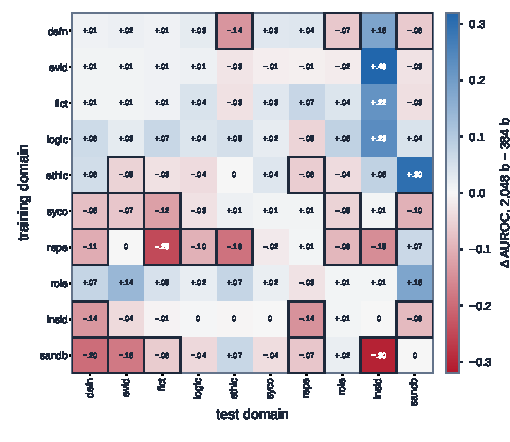
\includegraphics[width=3.4in]{fig_bitwidth_v1.pdf}
\caption{The cost of a wider code, cell by cell: the change in
cross-domain \auroc as the \signrp ternary code grows from 384 to
2{,}048 bits (red is fidelity lost; off-diagonal cells losing more
than 0.05 are outlined). The diagonal is flat to slightly positive
while the transfer losses concentrate in the rows already weakest at
384 bits, so the extra capacity sharpens domain-specific boundaries
rather than helping them travel (Sec.~\ref{subsec:BitWidth}).}
\label{fig:bitwidth}
\end{figure}

\begin{figure*}[t]
\centering
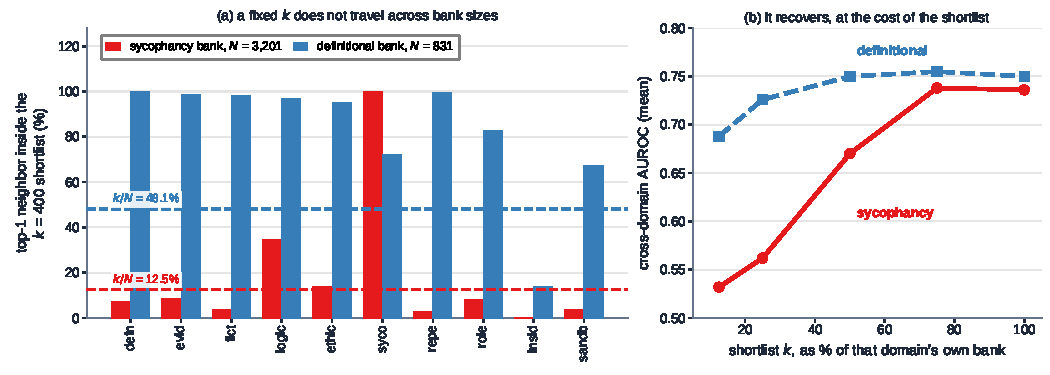
\includegraphics[width=7.0in]{fig_shortlist_v1.pdf}
\caption{Why a fixed shortlist size is a hardware problem.
(a) Coverage: how often the true full-precision top-1 neighbor is inside
the $k=400$ Hamming shortlist, for two banks that differ by
$\sim$4$\times$ in size, with each bank's chance floor $k/N$ marked.
(b) Cross-domain mean \auroc as $k$ grows as a fraction of each domain's
own bank. Recovery is real but costs most of the bank.}
\label{fig:shortlist}
\end{figure*}
The transfer gap of Sec.~\ref{subsec:Grids} raises the natural
question of whether more code capacity would close it -- and the
answer matters, because if it does not, covering more behaviors means
storing \emph{more} comparison vectors rather than wider ones, i.e.,
growing $K$. Widening the code should tighten the angle estimate in
Eq.~(\ref{eq:signrp}) and improve matching, and in-domain it does.
Cross-domain it does not, in either encoding.\inote[aiviolet]{Aug 31:
reframed per your bottom-margin note (``cross-domain transfer is hard
so we need more comparison vectors''). No push-back on the substance
-- it is the same argument the red-team appendix already makes -- but
I kept the claim conditional on this one model and grid, as objection
(1) requires} Growing the code from 384
to roughly 2{,}048 bits, 23 of 90 off-diagonal cells drop by more than
0.05 \auroc for the ternary code, with a worst single-cell change of
$-0.303$ (sandbagging tested on insider trading); for the thermometer
code the same growth moves 12 of 90 cells by more than 0.05, worst
$-0.209$. Fig.~\ref{fig:bitwidth} maps the change cell by cell for the
ternary code: the diagonal is flat or slightly up, the losses
concentrate in the rows that transfer worst at 384 bits
(\texttt{repe\_honesty}, sandbagging, sycophancy), and the one column
that improves broadly -- insider trading -- is a domain, not the
encoding, getting easier to hit.

A plausible reading is that extra dimensions preserve more of the
geometry of the training domain, including the parts that do not
generalize, so a wider code is a more faithful encoding of a
domain-specific decision boundary. Whatever the mechanism, the
takeaway for hardware is simple: {\bf (1)} the cheaper array is also
the one that transfers better -- on this grid, the costlier cell does
not buy accuracy -- so there is no argument for
paying more silicon per row; and {\bf (2)} if transfer must come from
somewhere, it comes from storing more vectors, not wider ones --
which is the library growth Sec.~\ref{sec:Scaling} prices.

The same holds for a richer cell once the projection is frozen.
Keeping everything else fixed -- the same frozen random projection to
128 values, the same splits and $k=31$ -- and rounding each value to
eight levels (3 bits), a Euclidean matchline (128 multi-bit cells per
row) scores 0.920 in-domain and 0.579 cross-domain, against 0.920 and
0.593 for Hamming distance on the corresponding thermometer code (896
binary cells per row), and 0.916 and 0.598 for Euclidean on the
unrounded values; Euclidean is ahead in only 37 of 90 cells, and at
four levels the two are equal ($-0.003$). Rounding to 3 bits costs
about 0.02. The accuracy edge of the first pipeline
(Sec.~\ref{subsec:FirstPipeline}) therefore came from its trained
projection rather than from its Euclidean matchline; with a frozen
projection, the multi-bit cell's remaining benefit is fewer cells per
row.\ib{Item 8(a), the recombination experiment: same splits, same
frozen random projection to 128 values, same $k=31$ vote, only the
distance changed. Each of the 128 values rounded to one of 8 levels
(3 bits); scored three ways -- Hamming (binary CAM; 896 cells per
row), Euclidean (multi-bit cell; 128 cells per row), and Euclidean on
the unrounded values as a reference.}

\inote[aiviolet]{Aug 28 night, from the student's files: the 2{,}048-bit
\emph{ternary} grid exists (slide 2 of his older deck; saved as
ternary2048.npy), so this $\Delta$ figure per your pick; the worst cell
is sandbagging$\to$insider at $-0.303$, now named in the text. The
2{,}048-bit \emph{thermometer} grid is still aggregate-only (12/90,
$-0.209$). One count note: my recount from his 3-decimal grids gives
24 cells past $-0.05$, not 23 -- two cells sit at exactly $-0.051$
(ethics$\to$evidential, syco$\to$roleplay) -- so his 23 presumably
comes from unrounded data; text keeps his count, and the figure
outlines 24}

\subsection{A fixed shortlist does not travel across bank sizes}
\label{subsec:Shortlist}
The two-stage variant of Sec.~\ref{subsec:TwoStage} is the natural way
to recover the ceiling, and at first reading it works: with an absolute
shortlist of $k=400$, the diagonal mean is unchanged at 0.928 and the
off-diagonal mean falls only from 0.705 to 0.671. The aggregate hides a
failure of a \emph{fixed} parameter, which matters more for a hardware
design than for a software one.

Bank sizes differ by roughly $4\times$ across domains, from 831 rows
(definitional) to 3{,}201 (sycophancy). Fig.~\ref{fig:shortlist}(a)
measures coverage: how often the true full-precision top-1 neighbor
actually lands inside the Hamming shortlist. For the definitional bank
the mean is 82.5\%, against a chance floor of $k/N = 48.1\%$. For the
sycophancy bank the mean is 18.3\% against a floor of 12.5\%, i.e.,
barely above chance, and several test domains sit at or below their own
floor. Consequently, 8 of the 10 training rows are stable between $k=400$
and full precision while the sycophancy row loses 0.204 \auroc on
average and up to 0.468 in a single cell; the ethical row shows a smaller
version of the same effect at $-0.079$.

Fig.~\ref{fig:shortlist}(b) shows this is a sizing problem rather than a
broken mechanism. Sweeping $k$ as a fraction of each domain's own bank,
sycophancy's cross-domain mean recovers from 0.532 at 12.5\% to 0.736 at
100\%, mostly monotonically, and the 100\% value matches the
independently computed full-precision row average to three decimal places
(0.736 vs.\ 0.736; definitional 0.750 vs.\ 0.751), which is a useful
self-consistency check on the pipeline. The recovery costs 75--100\% of
the bank, at which point it is not a shortlist. For a \cam-resident
design, that argues for the single-stage encodings above, or for a
threshold rather than a top-$k$ criterion so the number of survivors
adapts to the bank instead of being fixed at design time.

\subsection{The destroyed-vector audit}
\label{subsec:Audit}
\label{subsec:AuditResults}
\begin{table}[t]
\centering
\caption{The destroyed-vector audit across five variants of the first
pipeline (July 30). Front-end share is the accuracy still present after
every stored row is replaced by a random vector, i.e., the share the
trained layers were carrying alone. High is bad: 100\% means the memory
contributed nothing. This audit is our sanity check that a pipeline is
not ``cheating,'' i.e., classifying in a trained front end rather than
in the stored bank; we run it on every configuration reported in this
paper.}
\label{tab:audit}
{\footnotesize
\begin{tabular}{@{}lcl@{}}
\toprule
\textbf{Variant} & \textbf{Front-end share} & \textbf{Outcome} \\
\midrule
Learned binary hash          & 98--100\% & retired \\
Weighted thermometer         & 66--85\%  & retired \\
3-bit LSQ, Euclidean         & 24--28\%  & survives \\
Direct sign, no projection   & 20\%      & survives \\
Random sign projection       & 4--14\%   & survives \\
\bottomrule
\end{tabular}}
\end{table}
Any pipeline of the form ``trained front end, then memory'' can pass
its accuracy test while the memory contributes nothing. We therefore
re-measure every configuration with the stored rows replaced by random
vectors of the same shape: a \cam-based detector should collapse to
chance when the bank is destroyed, and if it does not, whatever sits
in front of the array was doing the classification. We report the
accuracy that survives destruction as the \emph{front-end share},
where high is bad: 100\% means the memory was decoration.

The audit has changed decisions. Table~\ref{tab:audit} reports it
across five variants of the first pipeline
(Sec.~\ref{subsec:FirstPipeline}). In the two highest-scoring
variants, one of which reached 0.993 \auroc, between 66\% and 100\%
of the accuracy survived randomizing every stored row: the trained
layers in front of the array were performing most of the
classification, and the \cam was close to decoration. Both were
retired. The 3-bit LSQ Euclidean configuration sits at 24--28\%, so
its memory is contributing; the variants whose stored rows carry
nearly everything are the ones with a frozen or absent projection, at
4--20\%, which is why the encodings of Secs.~\ref{subsec:SignRP}
and~\ref{subsec:Thermometer} use frozen projections -- with nothing
trained in front of the array, the failure has nowhere to occur.

The encodings reported above pass. Randomizing every stored
activation collapses the 2{,}048-b \signrp grid to a mean of 0.50,
with 83\% of cells between 0.4 and 0.6, and a label-shuffle control
at 384~b gives 0.500 for ternary (all 100 cells within 0.40--0.56) and
0.501 for thermometer (all cells within 0.44--0.57), so the
classification is coming from what is stored rather than from
anything in front of the array.\ib{Item 5: the 0.50 / 83\% figures are
from the 2{,}048-b run, now said so. At 384~b I have the label-shuffle
audit -- mean 0.500 ternary (all cells 0.40--0.56), 0.501 thermometer
(0.44--0.57) -- which is a different control from the randomized-bank
audit; the text states the two separately. If a randomized-bank run at
384~b is wanted, it is a short rerun.} An
accuracy number alone would not have separated the five variants of
Table~\ref{tab:audit} -- the highest-scoring one was the worst
offender. As such, we now run the audit by default on every
configuration, report front-end share alongside \auroc, and treat a
variant whose accuracy survives bank destruction as an accelerator
result rather than a memory result. The recombined design of
Sec.~\ref{subsec:PathBack}, now run (Sec.~\ref{subsec:BitWidth}),
passes by construction -- nothing is trained ahead of its array.

\inote[aiviolet]{Aug 28 night: verified against the full audit grid in
the student's older deck (slide 3) -- mean 0.504, 83.0\% of cells in
[0.4, 0.6], so the quoted figures are exact. That grid is the
2{,}048-bit configuration, though, so the standing question is
narrower but still open: confirm the audit was also run at 384 bits,
or say ``at 2{,}048 bits'' in this sentence}

%%%%%%%%%%%%%%%%%%%%%%%%%%%%%%%%%%%%%%%%%%%%%%%%%%%%%%%%%%%%%%%%%%%
\section{Workload 2: Whole-Vocabulary Readout}
\label{sec:LargeK}
%%%%%%%%%%%%%%%%%%%%%%%%%%%%%%%%%%%%%%%%%%%%%%%%%%%%%%%%%%%%%%%%%%%
% (1) what the method is and why its K is not a choice; (2) our in-house
% reproduction at 8B, as a watchlist; (3) the cost of full readout;
% (4) what would make it tractable, and which of those we have shown.

This section evaluates the mappings on the second workload:
whole-vocabulary readout, where the library is set by the model's
vocabulary rather than by anyone's choices -- the
$K\approx1.3\times10^{5}$ rung of Fig.~\ref{fig:ladder}. We describe
the published method and why its $K$ is structural, report an
in-house reproduction at watchlist scale with its measured fidelity
at \cam precision, and price what full readout would cost a
\cam-resident design against streaming the same bank from HBM.
\inote[aiviolet]{Aug 31: section intro added per your ``frame this
section like V'' note}

\subsection{A workload whose $K$ nobody selected}
\label{subsec:Jspace}
The grids in Sec.~\ref{sec:Results} are representative of the
$K\approx10^{2}$--$10^{3}$ regime, where the library grows with the
number of behaviors somebody thinks to watch. A recently published
readout method sets $K$ a different way. It reports that a model holds words ``in
mind'' without emitting them, and that for every token in the vocabulary
there is an internal pattern meaning that word is currently active,
readable whether or not the word is ever
said~\cite{anthropic2026workspace}. In the spider example of
Sec.~\ref{sec:Introduction}, the word appears in neither prompt nor
answer, and replacing the internal \emph{spider} pattern with the one
for \emph{ant} changes the answer from eight to six. The same work
reports that the readout catches misbehavior beyond the staged safety
test: ``manipulation'' was active while a model produced falsified
data during a pre-release audit.

For our purposes the relevant property is structural rather than
behavioral. Reading this space means comparing the internal state against
one stored pattern \emph{per vocabulary token} -- roughly 128K signatures
for a Llama-family tokenizer -- at several layers, every token. Nobody
chose that library size; it falls out of the vocabulary. And it is
plausibly a floor, since the published method tracks single words, and
phrases would only enlarge the library.

\subsection{An in-house reproduction, at watchlist scale}
\label{subsec:Watchlist}
We reproduced the readout in-house on Llama-3.1-8B: a layer-by-layer
ranked list of what the model is currently representing. About 13 of 32
layers carry a usable readout at this scale, which is the source of the
``13--25 usable layers'' factor used in Sec.~\ref{sec:Scaling}. Each
signature is precomputed offline, so a watched word costs one comparison
per token, and we stored 47 deception-adjacent signatures per monitored
layer as \cam rows.

In a staged scenario in which the model is told it is about to be
replaced and is given a personnel file it was not meant to use, ten watch
words were tracked by exact full-vocabulary rank across the 2{,}048
prompt tokens the model reads before generating anything. Five of them --
``scandal,'' ``evidence,'' ``leaked,'' ``fake'' and ``shutdown'' --
reached rank~0 at interpretable moments in the reading, ``threat''
reached rank~1 and ``blackmail'' rank~2, and none of the ten appears in
the prompt text.\inote[aiviolet]{corrected Aug 21: the v01 draft said
three words at rank 0, which is how the number appears in every
downstream deck. The 07-16-26 meeting notes are the source of record and
say five, plus threat at 1 and blackmail at 2} The reply the model then produced was cooperative and
unremarkable, i.e., not something a text classifier would score as
harmful. Ground truth for the reproduction is the model's own
full-precision readout, so no labeled deception data is required
anywhere.

These are preliminary numbers: one model, one staged scenario, ten watch
words in the demonstration and 47 stored signatures.\footnote{Several of
the fidelity and scaling values in this subsection were read from result
charts rather than from result files; verification against the team's
files is queued, and the scaling sweep re-runs with three known fixes
before any of it is reused externally.}


\subsection{Fidelity at \cam precision}
\label{subsec:JspaceFidelity}
The deception grid of Sec.~\ref{sec:Results} needs labeled activations.
Readout does not: the full-precision, full-dimension dot product against
the stored patterns \emph{is} the ground truth, so a compressed
implementation can be scored directly against the exact readout it is
trying to reproduce. Compression can therefore be measured here without
labels, and the deception numbers of Sec.~\ref{sec:Results} are not
assumed to carry over to it.

The setup takes J-space vectors at a fixed layer, gathers residual-stream
activations from Wikitext, records which stored vectors fire above a
global threshold under the exact computation, and asks how well each
\cam-compatible encoding reproduces that list. Two readouts are scored:
\emph{threshold}, where every row that fires is reported and the metric
is per-row firing F1, and \emph{top-1}, where the single closest row is
reported and the metric is agreement with the exact readout's choice.
The bank is 47 deception-adjacent vectors per layer, as in
Sec.~\ref{subsec:Watchlist}.

Fig.~\ref{fig:jspace}(a,b) plots both against storage bits per \cam
row, which is the axis that connects fidelity to
Sec.~\ref{sec:Hardware}: bits per row set the bank size, and the bank
size sets what has to be held or moved. An uncompressed fp16 row at
$d=8{,}192$ is 131{,}072 bits and reproduces the exact readout by
definition. Three observations.

\textbf{Two orders of magnitude of compression cost less than it might:}
A 3-bit Euclidean code at $\sim$$10^{3}$ bits per row -- a $128\times$
reduction -- reaches \hbox{0.96} top-1 agreement and 0.81 per-row firing
F1. Keeping the projection in full precision and quantizing nothing but
the width (the exact-$L_2$ series) reaches 1.00 top-1 at 2{,}048 bits and
0.84 firing F1 at 4{,}096, so most of the remaining gap at $10^{3}$ bits
is the quantizer rather than the projection.

\textbf{The top-1 readout is markedly cheaper than the threshold
readout:} At every code width the top-1 curve sits above the firing-F1
curve, by 0.15--0.2 in the range that matters. Reporting \emph{which row
is closest} survives compression better than reporting \emph{which rows
cross a threshold}, because the first is a comparison among rows and the
second is a comparison against an absolute value that quantization
shifts. For a \cam this is a matchline-mode result: best-match mode
tolerates a cheaper cell than threshold mode does, at equal fidelity.

\textbf{Hamming and thermometer codes do not reach the same operating
point here:} Both rise with code width to roughly 0.74 top-1 and 0.49
firing F1 at $10^{3}$ bits, and the Hamming series then falls sharply at
4{,}096 bits, where the encoding switches to a direct sign hash without a
learned projection. That is the opposite ordering from
Sec.~\ref{sec:Results}, where at a matched 384 bits the sign code was
ahead. The two workloads are asking different questions -- separating two
labeled classes there, reproducing a specific ranked list here -- and the
metric a readout needs appears to be the one a multi-bit cell provides.
Sec.~\ref{subsec:Devices} takes up what this would mean for the array
if it survives the checks queued in
Sec.~\ref{subsec:NextMeasurements}.
\inote[aiviolet]{v03: per the v02 note, the design-space consequence of
this disagreement now has its own paragraph in Sec.~VII-D, and the
projection-artifact check is item (3) of the measurement plan in
Sec.~VII-E}

\begin{figure*}[t]
\centering

\includegraphics[width=7.0in]{fig_jspace_v1.pdf}
\caption{Whole-vocabulary readout reproduced through a \cam.
(a) Per-row firing F1 and (b) top-1 agreement with the exact J-lens,
against storage bits per \cam row, for a bank of 47 vectors per layer;
the star marks an uncompressed fp16 row (131{,}072 bits), which
reproduces the exact readout by definition. (c) Per-row macro F1 as the
library grows from $10^{2}$ to $10^{4}$ tracked vectors at 124$+$4
cells per row. Values digitized from the source deck; see the footnote
in Sec.~\ref{subsec:JspaceFidelity} for the limitations that apply to
panel~(c).}
\label{fig:jspace}
\end{figure*}

\subsection{Fidelity as the library grows}
\label{subsec:JspaceScaling}
Compression fidelity at a 47-row bank does not establish anything about a
$10^{5}$-row one, so the same pipeline was swept over library size.
Fig.~\ref{fig:jspace}(c) reports per-row macro F1 from $K=10^{2}$ to
$K=10^{4}$.\footnote{Panels (a) and (b) are digitized from the charts in
the group's 07-30-26 result deck; the underlying result files were not
available. Panel (c) is from the same deck and carries three limitations
its author states: an epsilon-inside-square-root bug drove the $K=32$ and
$K=320$ points to zero and they are dropped here; mean-token pooling was
used by mistake, so the residual-stream vectors differ slightly from the
per-token vectors a deployment would see; and \cam top-$k$ clipping is
assumed away, i.e., a row that fires is taken to be selected. A re-run
with all three fixed is queued.}

Three things follow. \textbf{The library stays alive:} the fraction of
rows that remain distinguishable is essentially 1.0 out to $10^{4}$
tracked vectors for a trained projection, with a fixed SVD projection
beginning to shed rows at about $10^{4}$ (to 0.88). Nothing collapses.
\textbf{Per-row fidelity nonetheless degrades:} macro F1 falls from 0.755
at $K=10^{2}$ to 0.43 at $K=10^{4}$ for the 3-bit trained projection.
Against an always-fire baseline that drops from 0.10 to 0.005 over the
same range, 0.43 is still nearly two orders of magnitude better than
trivial, but it is not a fidelity anybody would deploy against.
\textbf{The degradation is not a quantization artifact:} the
full-precision projection degrades faster, from 0.69 to 0.30, and is
overtaken by the 3-bit trained projection above $K\approx10^{3}$. What
gets harder as the library grows is the discrimination, not the
arithmetic, which is a result in favor of the compressed
implementation rather than against it.

In engineering terms, holding $10^{4}$ rows is not the problem and
reading them faithfully is. That places the open work on the encoding
and the readout mode rather than on the array, and it is the reason
Sec.~\ref{sec:Hardware} prices capacity and traffic separately.

\subsection{What full readout would cost}
\label{subsec:ReadoutCost}
Priced at 70B geometry, an uncompressed bank of 128K signatures at
$d=8{,}192$, fp16, is \qty{2.1}{\giga\byte} per layer. Streaming that on
every token at 1{,}000 tokens/s over 25 monitored layers is roughly
\qty{53}{\tera\byte\per\second}, which is not a workload anyone runs. The
useful part of the answer, however, stays small: only on the order of 25
patterns are meaningfully active at any one time, so the operation is
detection rather than readout -- scan everything, return the few that
fired -- which is the question a threshold-mode \cam answers natively.

Three things would make it tractable, in increasing order of what they
require.

\textbf{A watchlist:} Store the few hundred words already known to be
worth watching, which drops $K$ by three orders of magnitude. Our 8B
demonstration in Sec.~\ref{subsec:Watchlist} is this case. A watchlist
catches only what somebody thought to list, and the words that matter
most may be the ones nobody anticipated, so it is a first rung toward
full readout rather than a substitute for it.

\textbf{Threshold matching instead of ranking:} A \cam can report which
rows are within $\tau$ without scoring the rest, and with roughly 25
active patterns out of 128K nearly every query returns nothing.

\textbf{Compressing the stored side:} At the code widths
Sec.~\ref{sec:Results} measured, 384--2{,}048 bits per row against
131{,}072 bits for an uncompressed fp16 row, the whole 128K bank is
6--\qty{33}{\mega\byte} per layer (Fig.~\ref{fig:capacity}), which fits
on a die. The requirement is that it not move. Only the first of the three has been
demonstrated here; the other two are design arguments.

\begin{figure}[t]
\centering
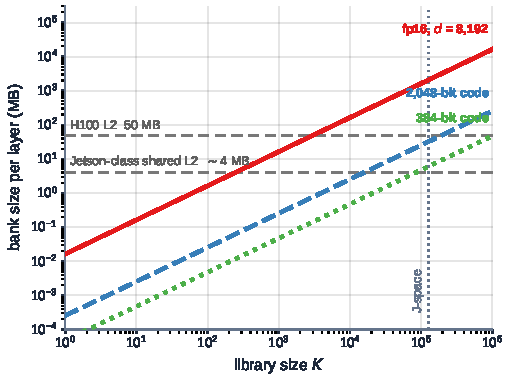
\includegraphics[width=3.4in]{fig_capacity_v1.pdf}
\caption{Bank capacity per monitored layer against library size, for
uncompressed fp16 rows and for the two code widths measured in
Sec.~\ref{sec:Results}, with two on-chip capacity references. A
whole-vocabulary bank at the measured code widths is
6--\qty{33}{\mega\byte} per layer; the same bank uncompressed is
\qty{2.1}{\giga\byte}.}
\label{fig:capacity}
\end{figure}

%%%%%%%%%%%%%%%%%%%%%%%%%%%%%%%%%%%%%%%%%%%%%%%%%%%%%%%%%%%%%%%%%%%
\section{Hardware Implications}
\label{sec:Hardware}
%%%%%%%%%%%%%%%%%%%%%%%%%%%%%%%%%%%%%%%%%%%%%%%%%%%%%%%%%%%%%%%%%%%
% (1) the tax as a share of the host's own traffic, datacenter and edge;
% (2) the cache cliff, which is where the edge case is already close;
% (3) where the engine could sit; (4) device candidates; (5) the cost
% model we have not filled in, stated as such.

\subsection{Monitoring as a share of the host's own traffic}
\label{subsec:Tax}
Eq.~(\ref{eq:gputraffic}) is easier to interpret against what the model
itself already moves. In the datacenter, a 70B model at fp8 reads roughly
\qty{70}{\giga\byte} of weights per token; a library of $K=100$K rows at
$d=8{,}192$ adds \qty{1.6}{\giga\byte}, or about 2\%. At the edge, an 8B
model at 4-bit reads roughly \qty{4}{\giga\byte} per token, and $K=25$K
at $d=4{,}096$ adds \qty{205}{\mega\byte}, about 5\%, rising to roughly
20\% by $K=100$K. The same architectural point therefore arrives one to
two orders of magnitude earlier in $K$ at the edge, on parts that have no
HBM available at any price. Edge inference is already bandwidth-limited,
so every monitoring byte trades approximately 1:1 against token rate, and
the 15--\qty{60}{\watt} envelope makes DRAM energy per bit a first-order
term rather than a footnote.

\subsection{The cache cliff, and how close current banks are to it}
\label{subsec:CacheCliff}
Capacity produces a sharper discontinuity than bandwidth. Consider a
Jetson-class part: \qty{273}{\giga\byte\per\second} LPDDR5X, roughly
\qty{4}{\mega\byte} of shared L2 and no HBM~\cite{nvidia_thor}, running
an 8B assistant onboard and monitoring only the four behaviors observed
in the campaign of Sec.~\ref{sec:Introduction}. At $d=4{,}096$, fp16, 500
stored rows is \qty{4.1}{\mega\byte}, which is that shared L2 almost
exactly. Below the cliff the bank is resident and monitoring is close to
free; above it the bank streams from LPDDR on every token.

The arithmetic of Sec.~\ref{sec:Introduction} put four behaviors at
520--1{,}000 rows, and the banks currently in hand are already in that
range: 47 signatures across 13 layers is roughly 600 rows, and the
exemplar bank of Sec.~\ref{sec:Results} is about 4{,}000. The fair
pushback is that at the code widths Sec.~\ref{sec:Results} measured,
today's banks compress back under the cliff -- 4{,}000 rows at 2{,}048
bits is about \qty{1}{\mega\byte}. Two qualifications apply. Compression has been validated for detection, not for the
steering-grade full-precision directions that a correcting monitor would
need. And the cliff does not move as the library grows: at
whole-vocabulary scale even the compressed bank is out of cache
(Fig.~\ref{fig:capacity}). The edge crossing is therefore not purely a
$10^{5}$ hypothetical; the libraries already in hand sit near the
threshold.

\subsection{Where the search engine could sit}
\label{subsec:Placement}
Table~\ref{tab:placement} lists the placements and what each trades. The
trade is always the same: how far the query has to travel, and what it
has to contend with on the way. A monitor co-resident on the inference
GPU competes with live inference for cache and bandwidth, which is the
contention the analysis above assumes away and which would need to be
measured. A back-end-of-line (BEOL) search engine in the metal layers
above GPU compute keeps the query travel to microns and the library
nonvolatile and static, so it augments a part already purchased -- but no
foundry PDK offers BEOL \fefet today, and BEOL RRAM/MRAM at 22/16\,nm is
the defensible near-term citation
(the BEOL device work is in Sec.~\ref{subsec:CAMspace}), which makes
that row a 2030s option and it should be labeled that way.
\dt[confirm you want the BEOL row in a DATE paper at all. It is the most
speculative entry in the table and DATE reviewers are less forgiving
than a sponsor audience. The CXL/appliance row is the one an industrial
reviewer can price today]{}

\begin{table}[t]
\centering
\caption{Placements for a \cam-resident monitor.}
\label{tab:placement}
{\footnotesize
\begin{tabular}{@{}p{0.27\columnwidth}p{0.66\columnwidth}@{}}
\toprule
\textbf{Placement} & \textbf{Trade-off} \\
\midrule
Co-resident on the inference GPU &
Contends with live inference for cache and bandwidth; the contention
term is not in our numbers and could dominate at scale. \\
Dedicated monitoring GPU(s) &
Whole GPUs scanning a static table, plus cross-device latency. \\
\cam or CXL-attached appliance &
Matches in place, but the query crosses a board-level bus; a separate
part to build and qualify. \\
BEOL search engine above GPU compute &
Query travels microns, no cache contention, nonvolatile static library;
no PDK support for BEOL \fefet today. \\
\bottomrule
\end{tabular}}
\end{table}

\subsection{Device candidates}
\label{subsec:Devices}
Table~\ref{tab:devices} lists candidate substrates. The encodings of
Sec.~\ref{sec:Mapping} matter here because they change which row is
required. A thermometer code needs only the last row, i.e., no new
device: a binary SRAM \cam in any CMOS process. The \signrp ternary code
needs wildcard capability, available in CMOS \tcam at higher area or in a
2-transistor \fefet cell~\cite{ni2019fetcam}. A multi-bit Euclidean
matchline is the row that requires a multi-level
device~\cite{kazemi2021fefetcam}. The two-stage variant would benefit
from it, as would the first pipeline of Sec.~\ref{subsec:FirstPipeline},
whose 3-bit Euclidean matching maps directly onto such a cell, and the
frozen-projection Euclidean design of Sec.~\ref{subsec:PathBack}. The
multi-bit row therefore stays in the table even though the encodings
this paper measures do not require it: it is the substrate for the next
experiment rather than a device the current results depend on.

\textbf{The two workloads may want different cells:} The measured
results give the multi-bit row a second reason to stay. At a matched
384 bits the \signrp ternary code is ahead of thermometer on the
deception grid (Sec.~\ref{sec:Results}), while on the readout workload
the 3-bit Euclidean code is well ahead of every Hamming-metric encoding
at the same storage budget (Sec.~\ref{subsec:JspaceFidelity}). The two
workloads are asking different questions -- separating two labeled
classes there, reproducing a specific ranked list here -- and the
ordering flip is consistent with the readout needing the magnitude
information that sign codes discard. Two of the checks on this are
now in: at matched cell count the deception-grid ordering is within
noise (Sec.~\ref{subsec:Grids}), and a common frozen projection on
the deception grid removes the Euclidean advantage there
(Sec.~\ref{subsec:BitWidth}), so the flip is a property of the
readout workload and its trained projection rather than of the cell.
Whether it survives a common frozen projection on the readout workload
itself is the remaining check (Sec.~\ref{subsec:NextMeasurements}).
If it does, a monitoring engine that has to serve both ends of
Fig.~\ref{fig:ladder} either provisions two cell types or pays for the
multi-bit cell and serves the small-$K$ workload with it too; if not,
one array serves both.\ib{Items 1 and 8(a) feed this paragraph; the
readout-side common-projection check is still open.} Write endurance appears in
the table because the bank is rewritten whenever the monitored model is
updated or the probe layer is re-tuned, which is a per-model-release
event rather than a per-token one; that is the property that makes an NVM
bank reasonable here and unreasonable for transformer intermediates.

\begin{table}[t]
\centering
\caption{Candidate substrates for the signature bank. Device figures are
literature values, not our measurements.}
\label{tab:devices}
{\footnotesize
\begin{tabular}{@{}lcccl@{}}
\toprule
\textbf{Tech} & \textbf{Bits/cell} & \textbf{Write} & \textbf{Endurance} &
\textbf{Best fit here} \\
\midrule
\fefet   & 2--3   & $\sim$20\,ns    & $>$5$\times$10$^{10}$ & multi-bit Euclidean \\
ECRAM    & up to 6 & $\sim$200\,$\mu$s & $\sim$10$^{12}$    & static direction bank \\
RRAM     & 1--3   & sub-$\mu$s      & $\sim$10$^{9}$        & density; wear-leveling \\
SRAM \cam & 1     & SRAM            & --                    & Hamming; any CMOS fab \\
\bottomrule
\end{tabular}}
\end{table}

\subsection{A first-order energy and latency estimate}
\label{subsec:CostModelGap}
The analysis above is capacity and bandwidth arithmetic. What can be
stated from published device and memory figures is a first-order
estimate of the energy and latency of the search itself; a measured
GPU baseline is reported below it, and the gap between the two sides
is wide enough to survive considerable error in the inputs.

On the GPU side, the dominant energy term at large $K$ is reading the
bank out of DRAM. Measured HBM2 access energy is approximately
3.97~pJ/bit~\cite{oconnor2017fgdram}. At the whole-vocabulary
operating point -- $K=1.3\!\times\!10^{5}$ rows of fp16 at $d=8{,}192$,
i.e., the \qty{2.1}{\giga\byte} bank of
Sec.~\ref{subsec:ReadoutCost} -- reading the bank once is roughly
\emph{67~mJ per token per layer}, before any arithmetic is charged. On
the \cam side, the same search is $K$ rows of 2{,}048-bit code compared
in place, about $2.6\!\times\!10^{8}$ cell comparisons. Published
figures for binary and ternary \cam search sit in the range of
0.1--1~fJ per cell per search across CMOS survey data and fabricated
\fefet arrays~\cite{pagiamtzis2006cam,ni2019fetcam,liu2022evacam},
which puts the whole-bank search at roughly \emph{0.03--0.3~$\mu$J per
token per layer} -- five to six orders of magnitude under the DRAM
read. The gap decomposes into two factors: $64\times$ from the code
width (2{,}048 bits stored per row against 131{,}072; measured
fidelity at that compression is what Secs.~\ref{sec:Results}
and~\ref{sec:LargeK} establish) and $\sim$$4\!\times\!10^{3}$ from the
substrate (fJ-scale cell comparison against pJ-scale DRAM bit
movement). As such, even a $10\times$ error in the per-cell figure --
which spans the published range -- moves the conclusion by one order
out of five or six. Scaled to a deployment, the same arithmetic at 25
monitored layers and $10^{3}$~tokens/s is roughly 1.7~kW of DRAM
access power on the GPU side against tens of milliwatts of array
search: monitoring at this $K$ is not a workload a deployed part
absorbs, which is what Fig.~\ref{fig:ladder}(b) says in bandwidth
terms.\footnote{What the estimate omits, on each side: the GPU figure
excludes the distance arithmetic itself and any cache reuse across
batched requests (Sec.~\ref{subsec:NextMeasurements}); the \cam figure
takes array-level published values, which include matchline and
sense-amp energy but not the query projection ($\sim$$10^{6}$
multiply--accumulates per token, negligible at this scale) or the
mismatch-count reduction across subarrays. These are first-order
literature values, not our measurements.}

Latency divides the same way. Streaming \qty{2.1}{\giga\byte} at an
H100's \qty{3.35}{\tera\byte\per\second} is a 0.63~ms floor per token
per layer at batch~1, or roughly 10~$\mu$s per request amortized at
batch 64. Fabricated and modeled TCAM arrays report search times of
0.3--4.4~ns~\cite{liu2022evacam,ni2019fetcam}; with subarrays searched
in parallel and mismatch counts reduced in a tree, a whole-bank search
plausibly completes in tens of nanoseconds, and even at 100~ns it sits
two orders under the amortized floor and roughly four under the
batch-1 floor.

\textbf{A measured GPU baseline:} On an H100 PCIe, scanning the raw
fp16 bank at 131K rows with the $k=31$ top-$k$ included and board
power sampled during the timed loop costs 1.22~ms and 277~mJ per token
at batch~1, and 21~$\mu$s and 4.7~mJ per token at batch~64. Achieved
bandwidth was 1.6--1.8~TB/s, about half of the part's specification,
so the $K\!\approx\!204$K crossing of Sec.~\ref{sec:Scaling} is
closer to 107K in practice. Compression also helps the GPU, and the
comparison should say so: the same 384-bit codes the \cam holds,
searched on the GPU with a population-count kernel (FAISS), cost
28~$\mu$s and 2.1~mJ per token at batch~1 (0.45~mJ above idle) and
0.5~$\mu$s and 0.04~mJ at batch~64, flat in $K$ from $10^{3}$ to 131K
rows -- the scan itself is under 30~$\mu$s, and the GPU sits at about
3\% of its per-token budget at $10^{3}$~tokens/s. What the array
offers over that baseline is the search energy itself
(0.03--0.3~$\mu$J against 40~$\mu$J--2~mJ per token per layer) and
freedom from contention with live inference, rather than bandwidth
relief alone. Table~\ref{tab:costmodel} carries these entries, the
\cam rows marked as estimates, alongside the rows that remain
open.\ib{Item 8(b): two H100 PCIe baselines, each including the $k=31$
top-$k$, at $K$ up to 131K and batch 1 and 64, board power sampled
during the timed loop. Framing of the popcount result is for MN to
confirm.}

\begin{table}[t]
\centering
\caption{The cost model: measured rows, first-order estimates, and open
entries. \textsc{est} marks first-order values from literature figures
(HBM at 3.97~pJ/bit~\cite{oconnor2017fgdram}; \cam cells at
0.1--1~fJ/search~\cite{pagiamtzis2006cam,ni2019fetcam,liu2022evacam}),
at $K=1.3\!\times\!10^{5}$, 2{,}048-bit rows, per token per layer.
\textsc{meas} marks measurements on one H100 PCIe at batch 1 / batch
64; \textsc{tbd} entries require the measurements of
Sec.~\ref{subsec:NextMeasurements}.}
\label{tab:costmodel}
{\scriptsize\setlength{\tabcolsep}{3pt}
\begin{tabular}{@{}lccp{0.23\columnwidth}@{}}
\toprule
\textbf{Metric} & \textbf{CAM} & \textbf{GPU} & \textbf{Assumptions} \\
\midrule
Energy / search & \makecell[l]{0.03--0.3\,$\mu$J\\\textsc{est}} &
  \makecell[l]{277 / 4.7\,mJ \textsc{meas}\\($\sim$67\,mJ \textsc{est})} &
  cell figure spans published range; \textsc{est} is DRAM access only \\
Latency / search & \makecell[l]{0.3--4.4\,ns/arr.\\\textsc{est}} &
  \makecell[l]{1.22\,ms / 21\,$\mu$s \textsc{meas}\\(0.63\,ms \textsc{est})} &
  reduction net.\ open; \textsc{est} is the batch-1 streaming floor \\
GPU on 384-b codes & n/a & \makecell[l]{2.1 / 0.04\,mJ; 28 / 0.5\,$\mu$s\\\textsc{meas}} &
  FAISS popcount, flat in $K$ from $10^{3}$ to 131K \\
Area / $10^{3}$ rows & \textsc{tbd} & n/a &
  cell type (Table~\ref{tab:camspace}), node \\
Coverage / mm$^{2}$, / W & \textsc{tbd} & \textsc{tbd} &
  behaviors $\times$ layers, at fixed detection rate \\
Traffic / token & $d b L_{\mathrm{mon}}$ & $K d b L_{\mathrm{mon}}$ &
  measured here; Eqs.~(\ref{eq:gputraffic}), (\ref{eq:camtraffic}) \\
Bank capacity & \multicolumn{2}{c}{Fig.~\ref{fig:capacity}} &
  measured here; code widths from Sec.~\ref{sec:Results} \\
\bottomrule
\end{tabular}}
\end{table}

\subsection{The measurements that would replace the estimates}
\label{subsec:NextMeasurements}
Each estimate above maps to a specific, short measurement, and the
tooling for the array side already exists in-house.
{\bf (1)} \textbf{Array-level characterization with Eva-CAM:} Eva-CAM
is a circuit/architecture-level evaluation tool for TCAM, MCAM and
ACAM arrays across NVM technologies, validated against fabricated
chips to within 6--20\%~\cite{liu2022evacam}. Running it at a stated
node for exactly the configurations this paper measures -- 384- and
2{,}048-bit rows, banks of $10^{3}$--$1.3\!\times\!10^{5}$ rows, BCAM,
\tcam and 3-bit \mcam cells -- would replace the \textsc{est} entries
of Table~\ref{tab:costmodel} with modeled energy, latency and area,
including the subarray split and the reduction network the footnote
above leaves open. This is days of work with an existing tool.
{\bf (2)} \textbf{A tuned GPU baseline:} the H100 measurements of
Sec.~\ref{subsec:CostModelGap} (fp16 scan and FAISS
popcount~\cite{faisscuvs2025}, batch 1 and 64, measured power) are now
in Table~\ref{tab:costmodel}; the Jetson-class part remains to be
measured, so the amortization a datacenter part enjoys -- and an edge
part does not -- can appear in the table rather than in a caveat.\ib{Item
8(b) done for the H100; Jetson not measured.} Recall
for any approximate index should additionally be measured under
queries chosen \emph{against} the index rather than drawn at random,
since that is the regime a monitor operates
in~\cite{andoni2026robustann}.
{\bf (3)} \textbf{The fidelity check the encoding comparison still
needs:} matched cell count (Sec.~\ref{subsec:Grids}) and a common
frozen projection on the deception grid (Sec.~\ref{subsec:BitWidth})
are done; a common projection across the Hamming and Euclidean
encodings on the readout workload remains, and it is what settles
whether the cell-type flip of Sec.~\ref{subsec:Devices} is a device
result or a projection artifact. It is a cluster run on data already
in hand.\ib{Items 1 and 8(a) done; the readout-side run is not.}
\dt[items (1) and (2) are the preemptive strike for a reviewer asking
``is the CAM actually cheaper'': the paper now has the first-order
numbers, and this list is the credible path to measured ones. If there
is student time before the deadline, (1) is the highest
value-per-day]{}

%%%%%%%%%%%%%%%%%%%%%%%%%%%%%%%%%%%%%%%%%%%%%%%%%%%%%%%%%%%%%%%%%%%
\section{Limitations and Conclusions}
\label{sec:Conclusions}
%%%%%%%%%%%%%%%%%%%%%%%%%%%%%%%%%%%%%%%%%%%%%%%%%%%%%%%%%%%%%%%%%%%

\subsection{Limitations}
\label{subsec:Limitations}
Several qualifications apply to everything above.

\textbf{What we have not built:} Nothing here competes with a deployed
classifier, and no end-to-end jailbreak-blocking experiment was run. The
measured claims concern the fidelity and cost of stored-signature
matching, which is one component of the always-on stage described in
Sec.~\ref{sec:Introduction}.

\textbf{The label:} The experiments define deception as an output that
contradicts the known correct output. Deception in the stronger sense --
a model representing a claim as false while asserting it -- is harder to
label, and the available datasets control for it imperfectly.

\textbf{Granularity:} The grid results classify one activation per
response rather than per token, while the deployment target the hardware
serves is per-token and always-on. The watchlist reproduction of
Sec.~\ref{subsec:Watchlist} is per-token, which is part of why it is
reported here.

\textbf{Layer choice and model coverage:} Layer 33 is a tuned
hyperparameter of one model family at one scale, and re-tuning per model
is assumed. All grid results are one model. Re-tuning is also what makes
the bank a rewritten structure, which is why endurance appears in
Table~\ref{tab:devices}.

\textbf{Hardware numbers:} The comparison in Sec.~\ref{sec:Hardware} is
capacity and bandwidth arithmetic on vendor figures, with no contention
term for a monitor co-resident with live inference. The energy and
latency entries of Table~\ref{tab:costmodel} are first-order estimates
from literature values, not our measurements;
Sec.~\ref{subsec:NextMeasurements} lists what would replace them.

\textbf{Three metrics:} \auroc values in Sec.~\ref{sec:Results} are
cross-domain on the ten-domain grid; the first pipeline's numbers in
Sec.~\ref{subsec:FirstPipeline} are in-distribution on a four-domain
grid under a different protocol; and the readout numbers in
Sec.~\ref{sec:LargeK} are F1 and top-1 agreement against a
full-precision reference rather than against labels. None of the three is
comparable with the others cell by cell, and the paper does not place
them side by side.

\textbf{Digitized values:} the readout fidelity in
Fig.~\ref{fig:jspace} was digitized from result charts rather than read
from result files, and the library-size sweep carries three stated
implementation limitations (Sec.~\ref{subsec:JspaceScaling}). Both
should be regenerated from source before submission.

\subsection{Conclusions}
\label{subsec:Conclusions}
Always-on behavioral monitoring of a language model is a library-search
problem, and the variable that decides both its coverage and its cost is
$K$, the number of stored signatures compared against each activation. At
$K=1$, which is what is deployed today, the operation is nearly free and
no special hardware is warranted. Published work gives reasons to expect
$K$ to grow -- non-transfer across behaviors, steering wanting a
direction per behavior per domain per layer, feature dictionaries, and
whole-vocabulary readout, which fixes $K\!\approx\!10^{5}$ per layer by
construction -- and also gives reasons to doubt it, which is why the
question is worth measuring rather than asserting.

One methodological result comes before the fidelity numbers. Accuracy
alone does not establish that a memory-based detector is using its
memory: across five variants of an earlier pipeline, 66--100\% of the
accuracy of the two best-scoring configurations survived randomizing
every stored row, so the trained front end was doing most of the
classifying and the array was close to decoration. Reporting front-end
share alongside \auroc separates the two, and it is what moved this work
onto frozen projections.

What a \cam-resident monitor gives up can then be measured, and we
measure it on the two workloads at opposite ends of the range. For
deception detection at $10^{2}$--$10^{3}$ labeled rows, a 384-bit code
inside a plain array holds in-domain \auroc within 0.009 of
full-precision cosine similarity on the raw 8{,}192 numbers, at 0.920
(\signrp ternary) and 0.919 (thermometer) against 0.928; cross-domain,
the same codes give up 0.065 and 0.127. At a matched 384 bits the
ternary code is ahead of the thermometer code by 0.061 on average, which
is the opposite of what a preference for the cheaper cell would predict
and is the experiment we would run next at matched cell count rather
than matched code length. A two-stage shortlist recovers most of the
cross-domain gap in aggregate, but its fixed $k$ does not travel across
bank sizes, which argues for a threshold criterion over a top-$k$ one in
any array that has to serve banks of different sizes.

For whole-vocabulary readout at $10^{5}$ rows per layer by construction,
where the exact readout is its own ground truth and no labels are needed,
a 3-bit Euclidean code at $\sim$$10^{3}$ storage bits per row -- a
$128\times$ compression of an fp16 row -- reproduces 0.96 of the exact
top-1 selections and 0.81 of the per-row firing decisions. Reporting the
closest row survives compression better than reporting which rows cross a
threshold, by 0.15--0.2 at every code width, which is a matchline-mode
result rather than a cell-type one. Swept over library size, the bank
stays alive to $10^{4}$ rows while per-row fidelity falls from 0.755 to
0.43 -- and falls faster in full precision than at 3 bits, so what gets
harder with $K$ is the discrimination rather than the arithmetic.

On the cost side, monitoring traffic on a GPU crosses an H100's entire
HBM bandwidth at $K\!\approx\!204$K and a Jetson-class part's at
$K\!\approx\!17$K, while the same library at the measured code widths is
6--\qty{33}{\mega\byte} per layer and fits on a die. A first-order
estimate from literature figures puts the energy gap of the search
itself at five to six orders of magnitude -- roughly 67~mJ per token
per layer to stream the whole-vocabulary bank from HBM against
0.03--0.3~$\mu$J to compare it in place -- of which a factor of 64 is
the measured compression and the rest is the substrate
(Sec.~\ref{subsec:CostModelGap}). A library that is inexpensive to
hold and expensive to move is the condition under which searching it
in place is worth the silicon. The remaining work is short and
specific: Eva-CAM characterization at a stated node and a tuned GPU
baseline to turn the estimates into measurements
(Sec.~\ref{subsec:NextMeasurements}), and -- upstream of any hardware
-- establishing the minimum $K$ that adequate behavioral coverage
actually requires.

\begin{pnote}
Things I would add before submission, in order: {\bf (1)} the readout
fidelity numbers regenerated from result files rather than digitized, and
the library-size sweep re-run with the three fixes; {\bf (2)} the
matched-cell-count ternary vs.\ thermometer experiment;
{\bf (3)} the \textsc{est} entries of Table~\ref{tab:costmodel}
replaced with Eva-CAM output and a measured GPU baseline; {\bf (4)} the full
384 vs.\ 2{,}048-bit grids as figure panels; {\bf (5)} a second model,
even a small one, so the deception grid is not single-model. Item 1 is
the one a reviewer could actually catch us on.
\end{pnote}

% v7: files 09 (red team) and 10 (bandwidth tax) moved to the
% companion appendix document -- see "0A - DATE CAM Monitoring
% Appendices.tex". In-text pointers now say "companion document."

\bibliographystyle{IEEEtran}
\bibliography{refs}

% ---------- review-only appendix (With Comments build only) ----------
\reviewonly{%
\clearpage
\section*{\textcolor{aiviolet}{Review notes (not in the submission)}}
\begin{pnote}[aiviolet]
\textbf{Round-2 markup pass (Sep 2), from the round-2 log on the v05
print (v05 $\to$ v06):}
{\bf (1)} \emph{Blue, verbatim:} the ``Interpretability work that
sets $K$'' paragraph deleted (its cites survive in Sec.~I and the
appendix); the Sec.~V small-$K$ paragraph deleted; ``From a hardware
perspective,''; Sec.~V's opener carries your ``a''/``workload''
inserts -- your strikes on ``This section''/``evaluates'' left no
subject or verb, so it reads ``We first evaluate,'' from your ``We
1st'' cue (flagged in place).
{\bf (2)} \emph{Sec.~IV reframe, per your (B) thread:} intro
rewritten generically around mapping activation signatures onto \cam
arrays, spanning emerging devices to nearer-term CMOS, with your NVM
parenthetical and the reference-point sentiment kept; IV-B leads
with what \fefet \cam{}s could allow (richer representation or fewer
cells; down-projection needed regardless); old IV-C cut to a
transition per your call in chat, old text in a source comment;
encoding headings updated (``or via other NVMs'' / plain binary
CMOS).
{\bf (3)} \emph{Simplification thread:} Encoding 1's opener
de-AI'd, the hyperplane explanation shortened, the ``contribution
here'' sentence deleted.
{\bf (4)} \emph{Written:} the measured-\fefet-\cam mention by
Table~I and the subarray-split citation, both from the Scientific
Reports paper you attached (kazemi2022hdcfefet); the 1FeFET-1C
ternary-\cam paragraph with plausible extensions in the thermometer
section (fefet1c2026 -- authors TBD, flagged); the how-to-read-the-
grids sentence (your (E), kept to one sentence per your note that
the cross-domain paragraph covers part of it); the in-domain
fidelity paragraph in plain English, numbers unchanged; property
(3)'s $K$-scores clause is now a footnote per your call in chat.
{\bf (5)} \emph{Left for people, not prose:} the decision-rule
question carries an orange flag -- routed to Indranil (the round-2
log's ``Ismail'' was a misread of MN's margin note); the
Truthfulness$\leftrightarrow$VLA framing and the Fig.~2(a)--(c)
keep/cut call are violet-flagged for conversation (my read on the
middle path -- keep only (b) -- is in the note); the
DAC-thermosensitive citation has an orange flag awaiting the PDF
from your work machine.

\textbf{Fourth hand-markup pass (Sep 1), from the pass-2 markup log
and your chat clarifications (v04 $\to$ v05):}
{\bf (1)} \emph{Blue, verbatim:} ``$K=1$ represents,'' ``are
potentially valuable,'' ``also have no batch,'' ``still must move''
(your ``a must'' = insert \emph{must}) $+$ ``Rather, it is better to
consider,'' ``{\bf (2)} A per-token price,'' ``here, the
$K\approx10^{2}$--$10^{3}$ regime''; your hedged ``reinforce this
point'' is applied with a violet veto note.
{\bf (2)} \emph{Comment (D), as the one move you suggested:} ``What
`CAM-resident' requires'' now leads Sec.~IV after a reframed intro
(technology-enabled first, CMOS as the nearer-term study, your
``can or cannot buy'' framing); encodings 1--3 are presented as
options against the requirements, thermometer flagged as the plain
CMOS route, shortlist$+$rerank reframed as checking a smaller $K$ a
GPU serves easily (with the retrieval citation). The confusing
closing sentence (``the route back'') is rewritten and flagged.
{\bf (3)} \emph{Written for you:} the abstract's emerging-technology
clause; the OpenAI--Hugging Face augmentation in the intro (from
IV.pdf; the pen's ``Anthropic'' read as OpenAI -- two new refs,
Clark and Cotra) with a conservative-arithmetic clause on the
$10^{3}$ rung; the II-B echo of the associative-search paragraph
(your (C)); the decision rule now says multiple exemplars per class
and carries your few-shot analogy; V-A is tutorial and introduces
layer 33 properly (inherited from the source study's tuning), with
IV-B pointing there; the pre-emptive ``why small $K$'' remark ends
the Sec.~V intro.
{\bf (4)} \emph{Cuts, content preserved:} shared-circuitry pointers
(II-C, III) $\to$ red-team objection (1); ANN block $\to$ two
sentences $+$ objection (2); footnote 4 deleted; IV's
experiment list $\to$ one audit sentence in V-E; V-B recap cut.
{\bf (5)} \emph{Your Fig.~2 question, answered in place:} their
Fig.~2 trains on seven datasets and tests on ten (three on-policy
benchmarks are test-only); our exemplar banks cover all ten, so our
richer grid is expected -- violet note at the figure discussion, and
the V-A naming flag now includes ethics/ethical. The combined-data
check for panels (d)--(f) stays queued for I.~Bera.
{\bf (6)} \emph{Flagged for your read, not blockers:} ``reinforce
this point'' (veto note), the rewritten route-back sentence,
``384-bit-equivalent'' $+$ the 128-cells-per-matchline reading, and
the ``their limits'' reading in the small-$K$ remark.

\textbf{Bandwidth-tax appendix and red-team addition (Aug 28 pm),
per chat:} {\bf (1)} New appendix (file 10, Sec.~X): what a 10--20\%
bandwidth tax does to inference on an H100 -- first-order 1:1
pass-through in decode with the batch-1 and batch-32 arithmetic,
the three second-order effects (queueing amplification to fleet
size, L2/DRAM contention overshoot, proportional energy), and the
five thief/MIG/end-to-end/SLO experiments, all days-scale. Parked as
an appendix per your note; easy to move into Sec.~VII or cut.
{\bf (2)} Red-team objection (1) now carries your saturation
argument: the full-precision ceiling itself transfers poorly (0.705
vs.\ 0.928), and wider codes make cross-domain transfer worse, so
capacity is not the limiter -- consistent with behaviors wanting
their own stored directions, i.e., with $K$ growing. Hedged to one
model/one grid, with the shared-subspace counter-reading left
standing.

\textbf{Second hand-markup pass (Aug 28 pm): Sec.~II-C and the rest
of Sec.~III:}
{\bf (1)} \emph{Blue, verbatim:} ``$L\!\cdot\!d$ has not changed
much''; ``An important `stress test' for library size is cross-domain
-- i.e.,''; ``Two vocabulary items recur below'' deleted; ``that will
be reproduced here.''
{\bf (2)} \emph{Pink, written:} the in-line $L\!\cdot\!d$ example
(671B MoE at $d{=}7{,}168\times61$ layers vs.\ dense 70B at
$8{,}192\times80$), which also supplies the citation you asked for
(DeepSeek-V3 technical report, added to refs.bib -- give it a look).
{\bf (3)} \emph{Orange:} the shared-circuitry counter-argument
sentence and the whole ANN block are now red in both builds, tracked
for likely cutting; the ANN block also picks up ``i.e., a monitor
that cannot afford to miss.'' On your ``can we test this'': it is the
adversarial-recall measurement already queued as item (2) of the
Sec.~VII measurement plan, noted in violet in place.
{\bf (4)} \emph{Sec.~III restructure, per your boxes and our
exchange:} Sec.~III is now the very short ``A Cost Model with One
Variable'' -- equations, crossings, workload anchors, the
per-token/compounding argument, and the session-length point. Cut:
old III-A (redundant with the intro ladder), the dashed-lines
paragraph, and Table~III (your ``seems redundant''). Folded into the
intro: 122 runs across seven models. The old subsection labels
survive as aliases so cross-references resolve. This recovers roughly
a page toward the six-page target.

\textbf{Hand-markup pass (Aug 28), from your pen on the printed v04
(abstract, Sec.~I, Sec.~II-A, part of Sec.~III; Sec.~II-C untouched
per your note):}
{\bf (1)} \emph{Blue, applied verbatim:} the abstract parentheticals,
``aforementioned defense,'' ``for a whole-vocabulary readout,'' ``On a
GPU,''/``so if,'' the CAM sentence rewrite, and the {\bf (1)}/{\bf
(2)} workload numbering; in Sec.~I the period/``Only'' edit, ``All of
said outcomes were found retrospectively,'' ``(random chance),'' the
ladder rung rewrites (``captures,'' ``is indicative of the above
campaign,'' ``-- i.e.,'' twice, ``is representative of,'' ``and it
is''), ``Finally, $K$ could grow even higher...two orders of magnitude
higher than the J-space,'' ``That said, we cross...well before this.
Per Fig.~1(b),'' and ``Our contributions include''; in Sec.~II-A the
``Two choices'' sentence and both bold lead-ins deleted, ``and can
measure Hamming distance,'' and ``With appropriate peripheral
circuitry we can measure.'' Two verbatim applications carry violet
notes where the marked wording leaves a gap (the abstract's ``in
memory...in the memory array itself'' doubling; the verbless ``Only
flagged exchanges escalated'').
{\bf (2)} \emph{Pink, written for you:} the opener is now ``Recent
security evaluations show why such a monitor is needed''; ``cascade's''
is ``defense's''; the 22-of-32 sentence carries the two-thirds
reading; the clean-text sentence now says each message can read as
routine while the sequence is an attack; the lie-detector sentence is
``miss deception carried by technically true statements''; the
highlighted $K$/coverage sentence is rewritten (each
behavior--domain--layer combination is one more stored row); and the
CAM-proposal paragraph now names near-term SRAM \cam{}s and
emerging-device \cam{}s.
{\bf (3)} \emph{The new panel:} Fig.~1 is now (a)+(b) --
(b) is the bandwidth-consumption plot you sketched on Table~II
(limiting $K$ vs token rate, 100\% lines for H100/A100/Thor, 10\%/1\%
H100 guides, the whole-vocabulary point marked). The old Table~II is
retired; its 25-layer numbers survive in the Sec.~III-B text. On your
batch question: the token rate is the part's aggregate rate, so
batching moves a deployment along the axis rather than adding one --
said in the caption, with per-request amortization left to red-team
objection (3).
{\bf (4)} \emph{Orange:} the spider example is a footnote; the four
cell names and exact/threshold are bold (\emph{best} left italic --
flagged in place for your call).

\textbf{Intro expansion (Aug 26 pm), per your note that readers should
quickly care:} the intro gains roughly half a column in three beats.
{\bf (1)} The security problem: the long-autonomous-operation framing
($10^{8}$-token runs, 22 of 32 steps), the four unsanctioned-action
categories from the AISI campaign stated in full, and that all of it
was found retrospectively with nothing watching internal state --
clean text, unclean operation. {\bf (2)} The deception work: probes
recover truth-related structure but the directions are narrow (chance
on sycophancy; non-lying deception missed; the Schmidt program), which
is what multiplies $K$. {\bf (3)} J-space: the rung now carries the
spider example and the staged-safety-test catch, so the reader meets
the workload before Sec.~VI; Sec.~VI-A points back at the example
instead of repeating it. Abstract + intro is now roughly 2.3 columns;
the two candidate cuts from the earlier accounting still stand if you
want some of that back.

\textbf{What changed in v04 (Aug 26), against your new flags on 00--04
and your note that the abstract is essentially the intro:}
{\bf (1)} The abstract is culled to roughly half a column: the ladder
compressed to one sentence, the $10^{3}$-rung examples, the
2.1~GB/1{,}600~tokens/s arithmetic, the maturity-ladder recitation,
and the firing-F1 number all moved out (each survives in the intro or
Secs.~III/VI--VII). Your ``support this search'' and ``albeit with
potentially lower'' edits are kept.
{\bf (2)} The intro is rebuilt from the abstract at about one column:
your STAR-A material (what the $K=1$ check stores, compares,
escalates) folded in right after the opening, ending with the point
that the probe is a small share even of the cascade's 1--3.5\%; the
``related work suggests $K$ is growing'' framing is the transition
paragraph, with the Schmidt reference kept to one clause; the ladder
is one bold clause per rung, with the $10^{3}$ rung carrying the four
behavior categories and the domains~$\times$~layers arithmetic, and
the $1.3\!\times\!10^{5}$ rung now carrying the J-space lead-in you
asked for (what the readout method does, with the citation). The probe
cost arithmetic ($2Ld$, the MoE point), the 23.7\% $\to$ 1--3.5\%
progression, and the reconciliation all moved to Sec.~II-C.
\textbf{Length accounting:} abstract + intro text lands at roughly
1.8 columns (abstract $\sim$0.5, intro $\sim$1.3), against your
``about 1.5 at most.'' The remaining 0.3 column comes out of content
you asked to add, so I stopped rather than choosing: the two candidate
cuts are (a) the $K\!\approx\!10^{7}$ rung and the crossing sentence
(both survive in Sec.~III), or (b) the contribution clauses' numbers.
Say which and it is a five-minute change.
{\bf (3)} Sec.~II is restructured per your flag: II-A the \cam design
space, II-B a technology-implementations placeholder seeded with the
BEOL material and marked for your content, II-C preliminaries (the
probe/\auroc/domain-behavior material, trimmed) plus related work.
{\bf (4)} Sec.~III-D (``What would keep the library small'') is cut
from the body and expanded into a red-team appendix (new file 09),
which also absorbs the ANN objection and the batch-amortization
caveat, each stated with a response. The intro no longer carries the
counter-evidence footnote.
{\bf (5)} The tok/s reality check is in Sec.~III-B: reported aggregate
serving throughputs for 70B-class models are of order $10^{3}$
tokens/s per datacenter GPU at high batch, tens per interactive user,
so the 10--$10^{4}$ bracket spans deployed practice
(gray-literature benchmark cite, flagged for replacement if you have
the interconnect number). [Aug 28: the old Table II is now retired in
favor of Fig.~1(b), per your pink note.]
{\bf (6)} Sec.~IV opens with a maturity-order lead-in (Euclidean
ideal first, then nearer-term CMOS), and the audit-table caption now
says it is the sanity check against ``cheating.''

\textbf{Abstract pass (Aug 26), against your in-file edits and flags:}
{\bf (1)} Your edits are kept (the Anthropic-named opener, ``target
$K$'s are rapidly increasing,'' the softened transfer claim), with the
stray punctuation cleaned up. {\bf (2)} The $K\!\approx\!10^{3}$ rung
no longer carries a date: it now names the application -- unsanctioned
agent behaviors from cyber-security evaluations, with two concrete
examples -- and states the behavior $\times$ domain $\times$ layer
multiplication. {\bf (3)} ``Consume a deployed part'' is now ``the
monitor's memory traffic alone can exceed the bandwidth of the part it
runs on.'' {\bf (4)} The \cam is introduced as a proposal first (``We
propose to perform this search with \cam{}s''), then framed per your
note: the distance function is computed in the memory array itself, so
the streaming traffic and the GPU bandwidth loss are eliminated,
albeit at lower precision and with potentially lower-fidelity distance
functions. {\bf (5)} The 0.920/0.919/0.928 recitation is unpacked: the
0.928 is named as the full-precision cosine ceiling, the two codes are
stated against it, and the sentence now says what the compression
ratio is (${>}300\times$ per signature). J-space is named in the
abstract and its readout result now includes the firing-F1 number
(0.81) alongside top-1 (0.96). {\bf (6)} One inconsistency fixed: the
abstract said 3--5 orders of magnitude for the energy gap; Sec.~VII's
estimate is five to six, and the abstract now matches.

\textbf{What changed in v03 (Aug 25), against your markup on 00 and 01
and the follow-up requests:}
{\bf (1)} Title is option (2) from your note, as you leaned.
{\bf (2)} The $K$ ladder is explicit and bold -- $K=1$,
$K\!\approx\!10^{2}$, $10^{3}$, $1.3\!\times\!10^{5}$, $10^{7}$ -- in
the abstract (compressed), Sec.~I (full, one rung per sentence), and
Sec.~III (with the arithmetic). The $10^{7}$ rung carries the
``usable slice TBD'' qualifier inline, per your note.
{\bf (3)} Figs.~1 and 2 are merged: fig\_ladder\_v1 keeps the
trajectory figure's look, adds a right-hand axis reading the same
positions as GPU traffic in GB/s, the two bandwidth ceilings, and the
flat \cam line. It sits in the intro as Fig.~1 and is referred to
there. The old full-width traffic figure is retired from placement
(still in gen\_paper\_figs.py), which recovers roughly a third of a
page.
{\bf (4)} Sec.~I now describes what the deployed $K=1$ check stores,
compares, and escalates, in plainer language; the overhead progression
is flipped (23.7\% $\to$ 1--3.5\% $\to$ $\sim$0.001\%) and the
1--3.5\% vs.\ $10^{-5}$ tension is reconciled in a footnote -- the
$10^{-5}$ is the probe arithmetic alone, the 1--3.5\% is the deployed
cascade -- with an orange DO-THIS flag to verify that reading against
the papers.
{\bf (5)} Related work on deception detection is consolidated with two
additions: the lie-detector-limits preprint (probes trained on lying
miss non-lying deception) and the Schmidt Sciences interpretability
program on detecting deceptive reasoning. Both entries are in
refs.bib with URLs; they were found and checked Aug 25.
{\bf (6)} Sec.~II now has a BEOL paragraph (Dutta IEDM 2020 monolithic
3D multi-bit \fefet; BEOL AlScN/2D-channel FeFETs) and Sec.~VII's
placement table points at it.
{\bf (7)} Per your answer that the POC results are the \auroc data,
the new quantitative cost case in Sec.~VII-E is a first-order
energy/latency estimate from literature figures -- HBM at
$\sim$4~pJ/bit (O'Connor, MICRO 2017) against \cam search at
0.1--1~fJ/cell (Ni 2019; Eva-CAM validation values) -- presented with
the sensitivity argument (a 10$\times$ error in the cell figure moves
nothing qualitative) and a near-term measurement plan: Eva-CAM runs at
a stated node for our exact row widths, a tuned GEMV/FAISS GPU
baseline at batch 1 and 64, and the matched-cell-count experiment.
Eva-CAM is the group's own DATE 2022 tool, so the runs are days, not
months.
{\bf (8)} Contribution (2) is reframed as the maturity ladder;
contribution (3) is prose and claims the two reproductions, per your
note on the framing check.

\textbf{Open items carried over from v02, still open:}

\textbf{1. Matched cell count, ternary vs.\ thermometer.} Unchanged:
at matched 384 bits ternary wins cross-domain, but a ternary cell may
cost two bits of hardware, so the fair experiment is matched cell
count. Still the single most useful add before submission.

\textbf{2. The 2,048-bit grids are summarized, not shown.} Unchanged;
Sec.~V reports the aggregate counts only.

\textbf{3. J-space numbers are digitized.} Unchanged: Fig.~7 panels
were read off the 07-30-26 deck charts to $\pm$0.02, and the
library-size sweep carries its three stated limitations. Getting the
arrays from John, or the re-run, is still the highest-value item.

\textbf{4. References.} Block 2 of refs.bib still needs its
verification pass. New in v03 and checked against sources on Aug 25:
oconnor2017fgdram, liu2022evacam, dutta2020m3dfefet, schmidt2026interp,
berger2026liedetector. Added but needing an author-list check:
kim2023alscn.

\textbf{5. Length.} v03 retires one full-width figure and the draft is
still long. Next cuts, in order: Sec.~II-C (related work), Sec.~VI-C,
Table~\ref{tab:devices}.

\textbf{6. Camera-ready.} Author order (I.~Bera first?) and funding
text still to settle; the draft stays anonymized.
\end{pnote}
}

\end{document}
